\documentclass[../../../main]{subfiles}
\begin{document}

\section{結果}


\subsection{レーザー光による回折強度パターンの測定}

\subsubsection{スリットの形状の計測結果}\label{subsubsec:slit_shape}
使用したスリットの形状は図\ref{fig:slit_image}の通りである。
図\ref{subfig:measure}は、画像のピクセルと実際の大きさを対応させるために、最小メモリが \SI{0.01}{mm} の定規をおいて撮影したものである。
このメモリを用いて、計測すると\SI{0.90}{mm}が\SI{772.093}{pixel}に対応した。
したがって、\SI{1.17}{um/pixel}であると計算された。
これを用いて各スリットの形状を計測した結果を表\ref{tab:circle_slit_diameter}、表\ref{tab:ss_slits}、表\ref{tab:ds_slits}に示す。

%Please add the following packages if necessary:
%\usepackage{booktabs, multirow} % for borders and merged ranges
%\usepackage{soul}% for underlines
%\usepackage{xcolor,colortbl} % for cell colors
%\usepackage{changepage,threeparttable} % for wide tables
%If the table is too wide, replace \begin{table}[!htp]...\end{table} with
%\begin{adjustwidth}{-2.5 cm}{-2.5 cm}\centering\begin{threeparttable}[!htb]...\end{threeparttable}\end{adjustwidth}
\begin{table}[!htp]\centering
	\caption{円スリットの直径}\label{tab:circle_slit_diameter}
	\scriptsize
	\begin{tabular}{cc}\toprule
		px     & \si{\micro\meter} \\\midrule
		230.12 & 268.24            \\
		\bottomrule
	\end{tabular}
\end{table}

%Please add the following packages if necessary:
%\usepackage{booktabs, multirow} % for borders and merged ranges
%\usepackage{soul}% for underlines
%\usepackage{xcolor,colortbl} % for cell colors
%\usepackage{changepage,threeparttable} % for wide tables
%If the table is too wide, replace \begin{table}[!htp]...\end{table} with
%\begin{adjustwidth}{-2.5 cm}{-2.5 cm}\centering\begin{threeparttable}[!htb]...\end{threeparttable}\end{adjustwidth}
\begin{table}[!htp]\centering
	\caption{単スリットの形状}\label{tab:ss_slits}
	\scriptsize
	\begin{tabular}{ccc}\toprule
		    & slit width / px & slit width / \si{um} \\\midrule
		SS1 & 36.892          & 43.004               \\
		SS2 & 74.169          & 86.456               \\
		SS3 & 111.113         & 129.520              \\
		\bottomrule
	\end{tabular}
\end{table}

%Please add the following packages if necessary:
%\usepackage{booktabs, multirow} % for borders and merged ranges
%\usepackage{soul}% for underlines
%\usepackage{xcolor,colortbl} % for cell colors
%\usepackage{changepage,threeparttable} % for wide tables
%If the table is too wide, replace \begin{table}[!htp]...\end{table} with
%\begin{adjustwidth}{-2.5 cm}{-2.5 cm}\centering\begin{threeparttable}[!htb]...\end{threeparttable}\end{adjustwidth}
\begin{table}[!htp]\centering
	\caption{デュアルスリットの形状}\label{tab:ds_slits}
	\scriptsize
	\begin{tabular}{cccccccc}\toprule
		    & slit 1 width / px & slit 2 width / px & slit distance / px & slit 1 width / \si{\micro\meter} & slit 2 width / \si{\micro\meter} & slit distance / \si{\micro\meter} \\\midrule
		DS1 & 49.313            & 48.545            & 130.750            & 57.482                           & 56.587                           & 152.410                           \\
		DS2 & 71.609            & 69.674            & 131.673            & 83.472                           & 81.216                           & 153.486                           \\
		DS3 & 71.007            & 70.007            & 331.020            & 82.770                           & 81.605                           & 385.858                           \\
		\bottomrule
	\end{tabular}
\end{table}

\begin{figure}[htbp]
    \centering
    \begin{minipage}[ht]{0.48\hsize}\centering
        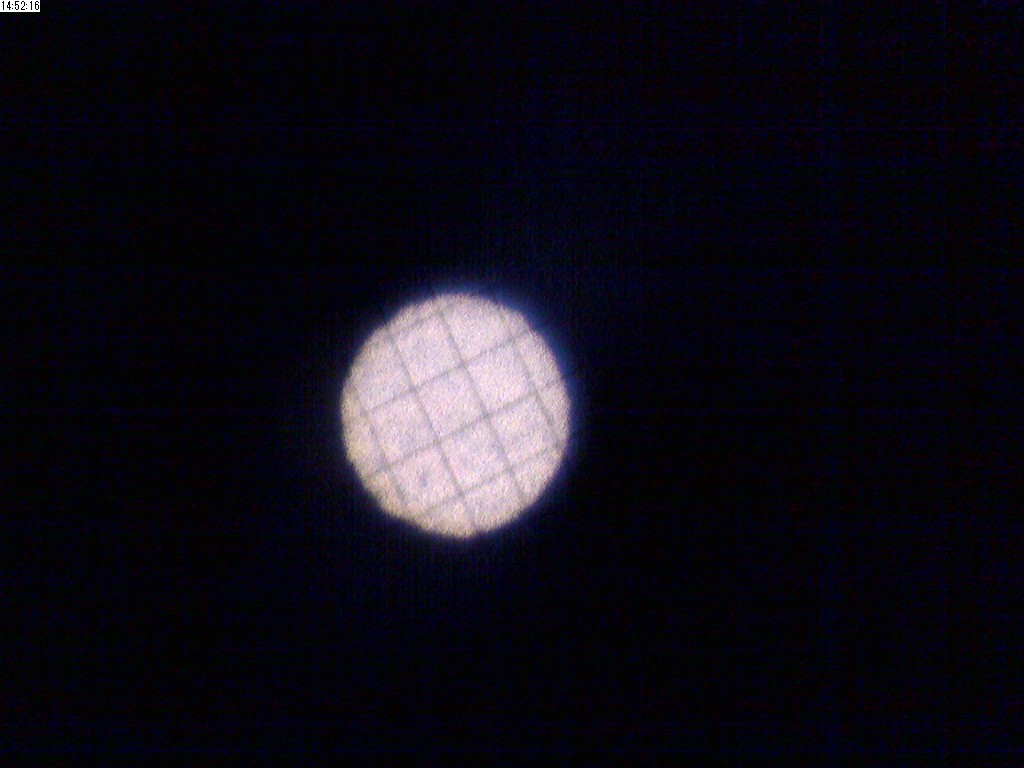
\includegraphics[width=\linewidth]{src/figures/result/circle_slit.jpg}
        \subcaption{円スリット}\label{subfig:circle_slit}
    \end{minipage}
    \begin{minipage}[ht]{0.48\hsize}\centering
        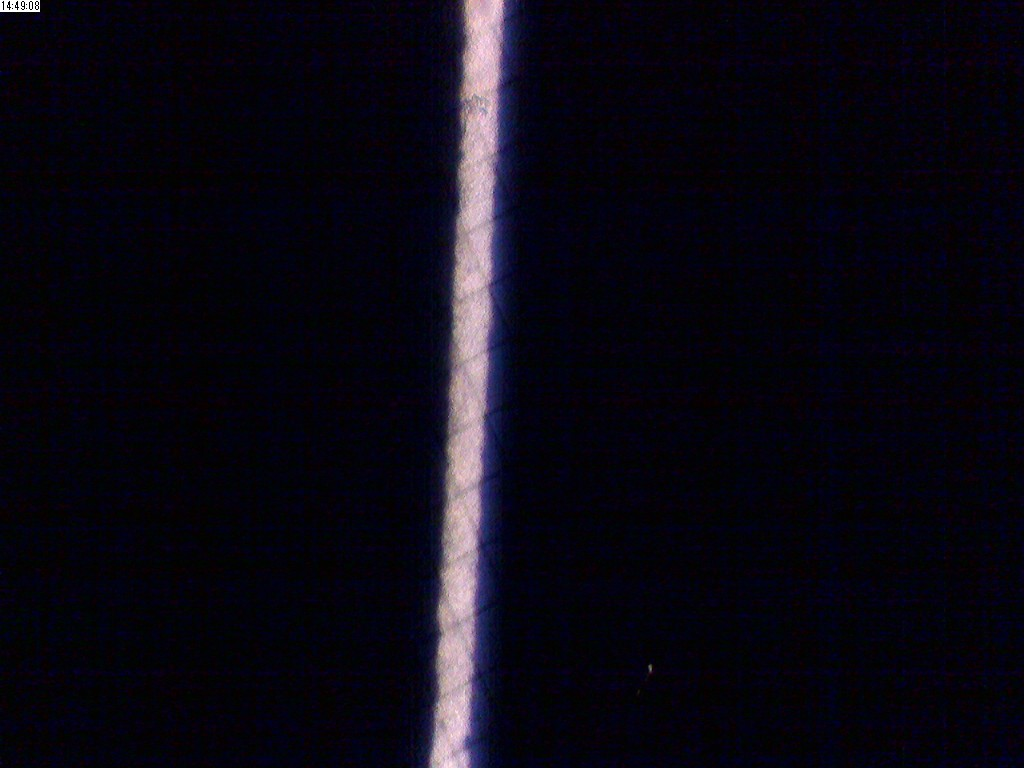
\includegraphics[width=\linewidth]{src/figures/result/ss1_slit.jpg}
        \subcaption{単スリット1}\label{subfig:ss1_slit}
    \end{minipage}
    \begin{minipage}[ht]{0.48\hsize}\centering
        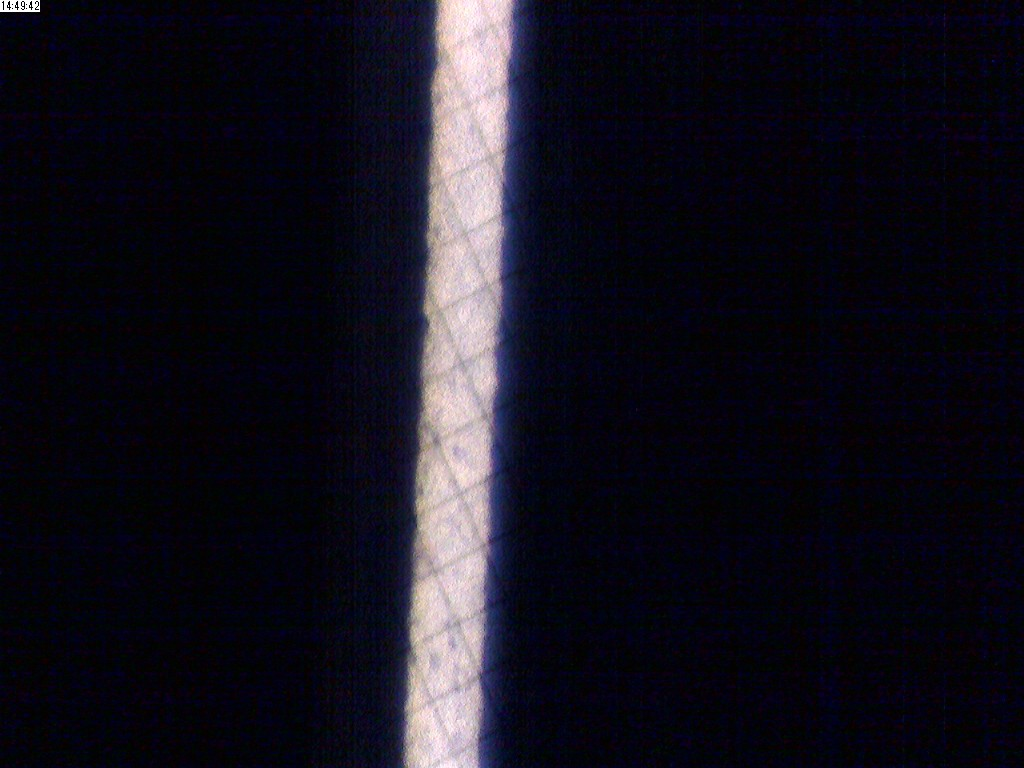
\includegraphics[width=\linewidth]{src/figures/result/ss2_slit.jpg}
        \subcaption{単スリット2}\label{subfig:ss2_slit}
    \end{minipage}
    \begin{minipage}[ht]{0.48\hsize}\centering
        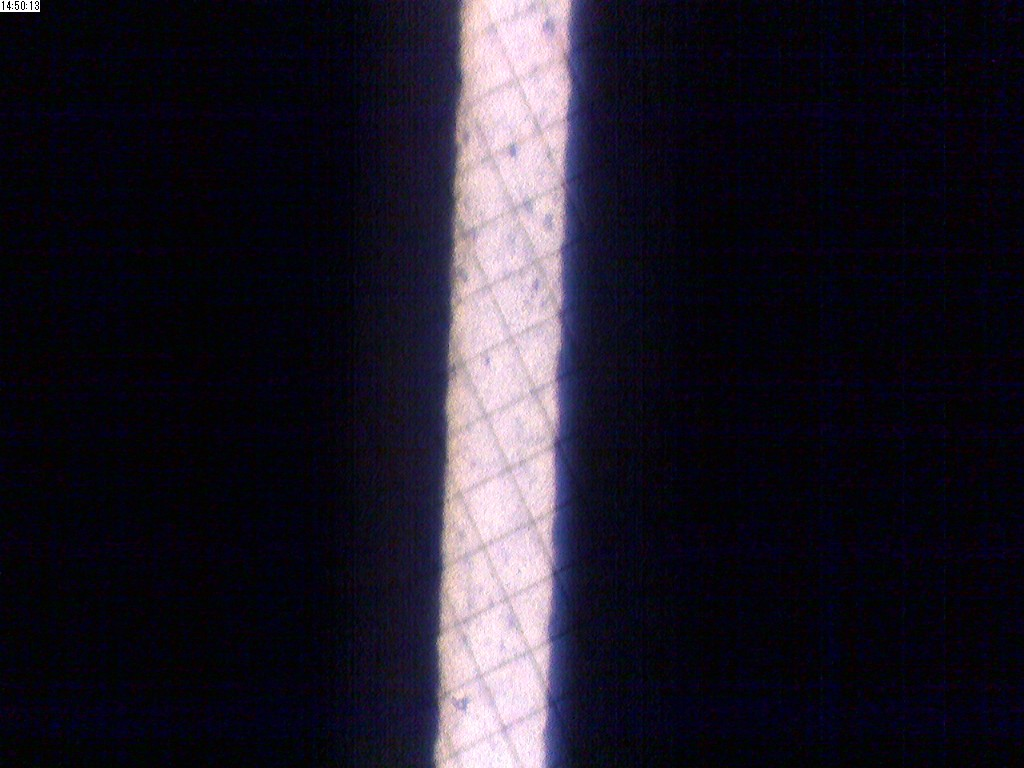
\includegraphics[width=\linewidth]{src/figures/result/ss3_slit.jpg}
        \subcaption{単スリット3}\label{subfig:ss3_slit}
    \end{minipage}
    \begin{minipage}[ht]{0.48\hsize}\centering
        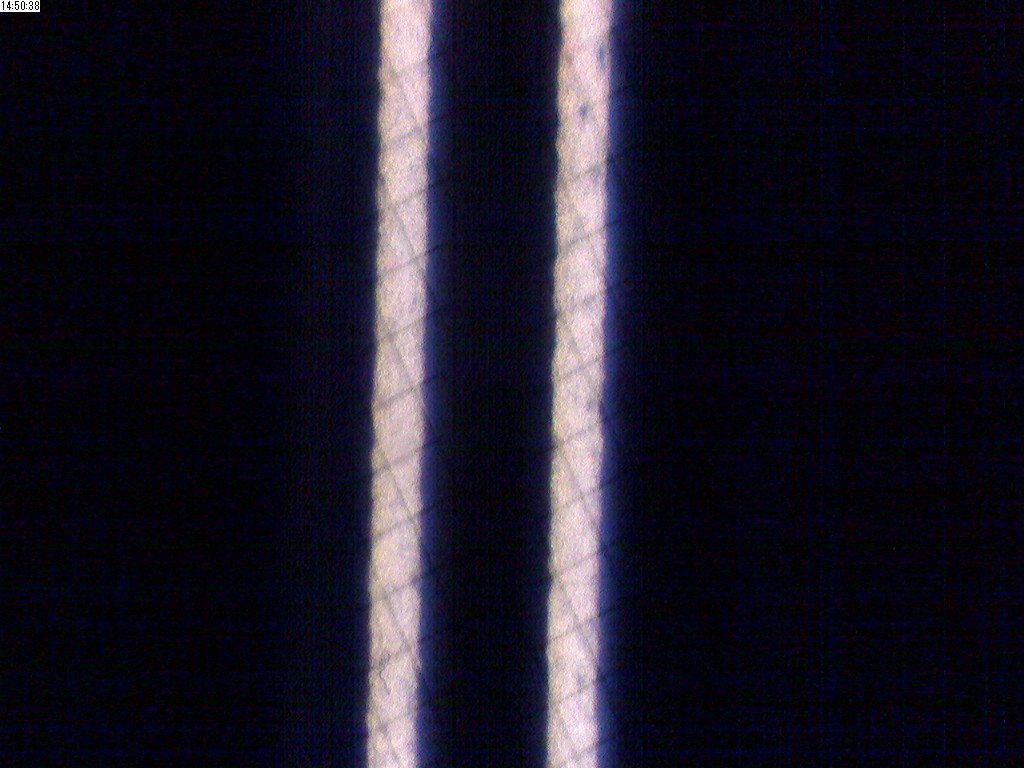
\includegraphics[width=\linewidth]{src/figures/result/ds1_slit.jpg}
        \subcaption{ダブルスリット1}\label{subfig:ds1_slit}
    \end{minipage}
    \begin{minipage}[ht]{0.48\hsize}\centering
        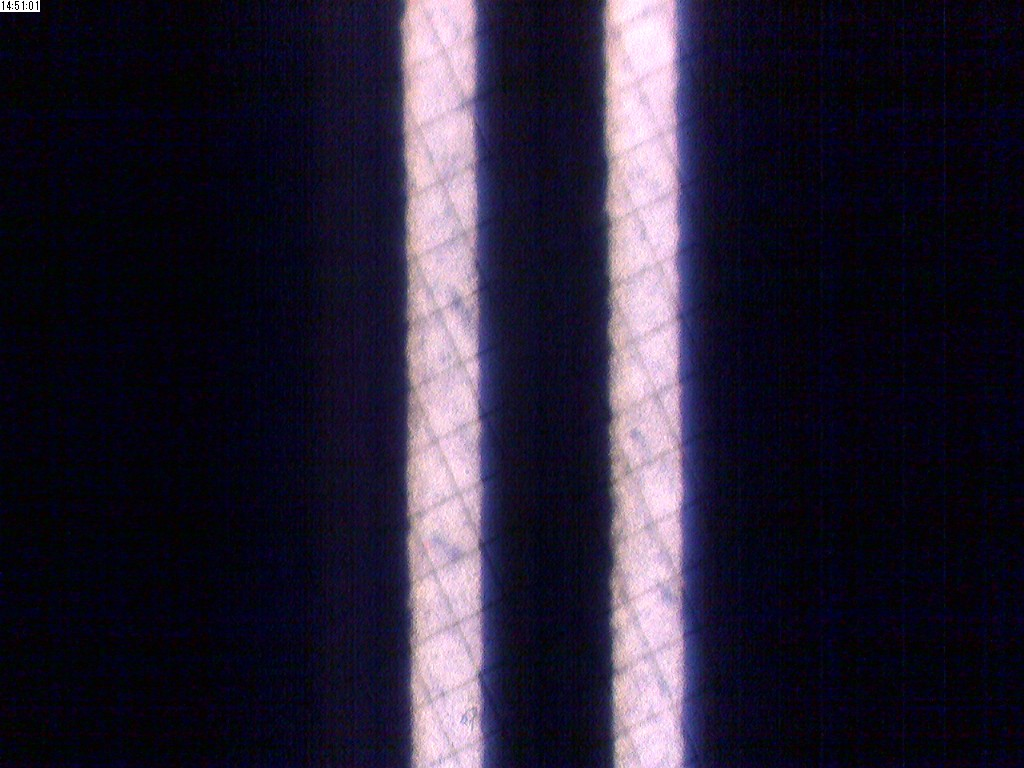
\includegraphics[width=\linewidth]{src/figures/result/ds2_slit.jpg}
        \subcaption{ダブルスリット2}\label{subfig:ds2_slit}
    \end{minipage}
\end{figure}
\begin{figure}[htbp]
    \centering
    \addtocounter{figure}{-1}
    \begin{subfigure}{0.48\hsize}\centering
        \addtocounter{subfigure}{6}
        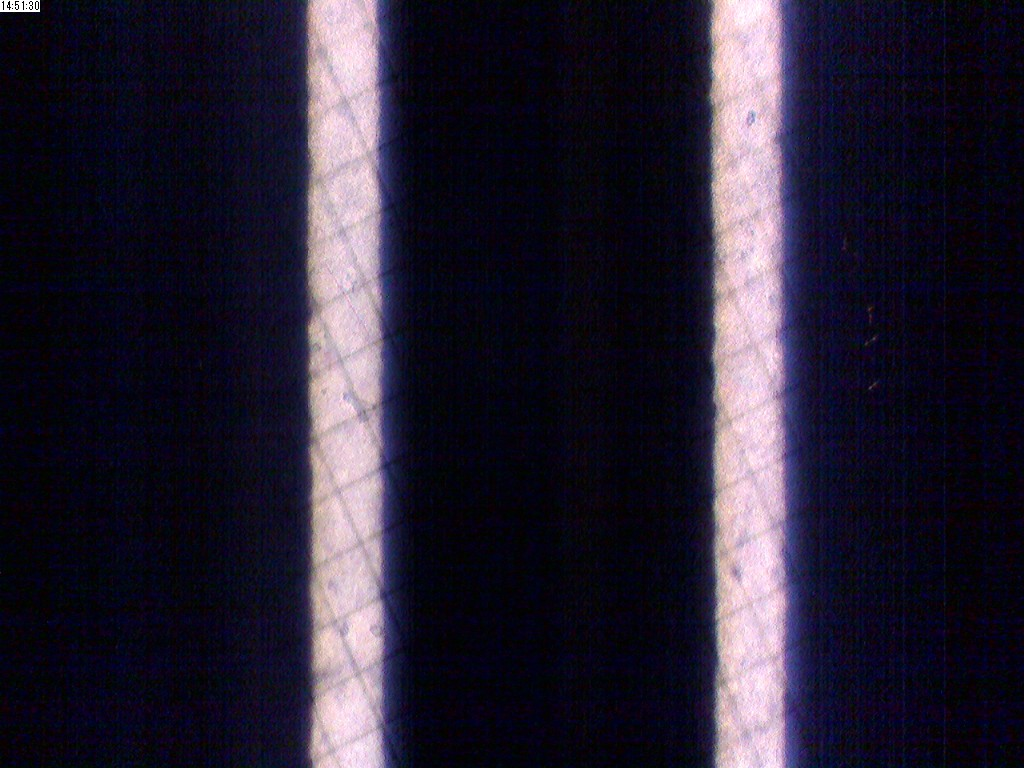
\includegraphics[width=\linewidth]{src/figures/result/ds3_slit.jpg}
        \subcaption{ダブルスリット3}\label{subfig:ds3_slit}
    \end{subfigure}
    % \begin{subfigure}{0.48\hsize}
    %     \includegraphics[width=\linewidth]{src/figures/result/square.jpg}
    %     \subcaption{正方形}\label{subfig:square_slit}
    % \end{subfigure}
    % \begin{minipage}[ht]{0.48\hsize}\centering
    %     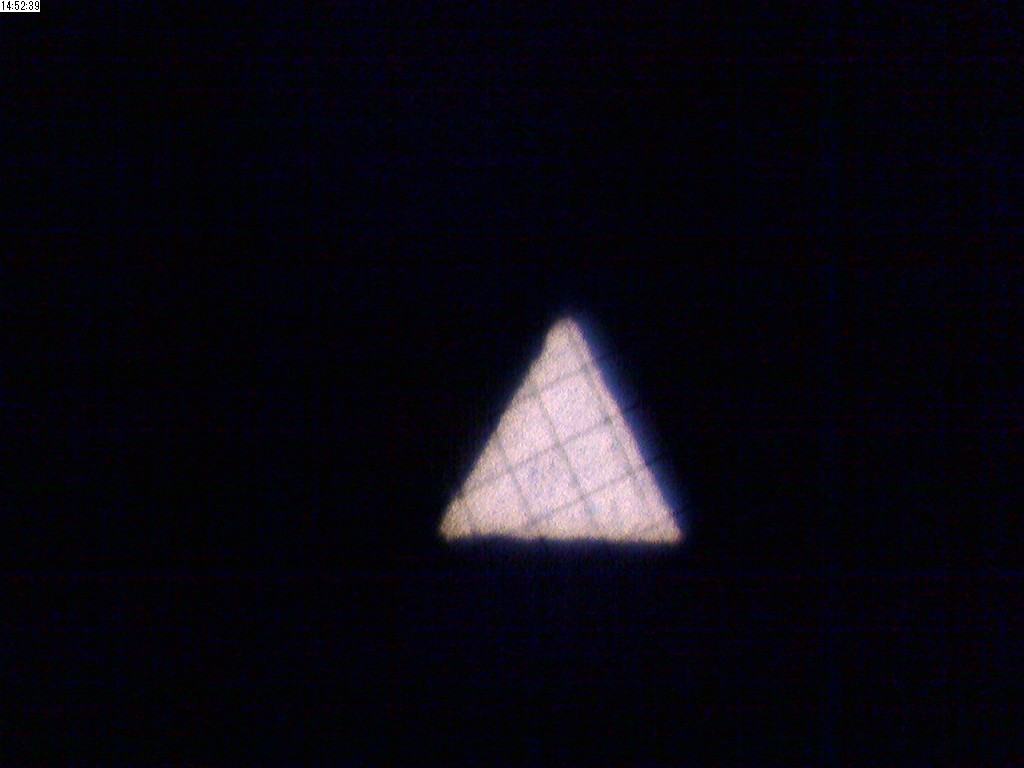
\includegraphics[width=\linewidth]{src/figures/result/triangle_slit.jpg}
    %     \subcaption{三角形スリット}\label{subfig:triangle_slit}
    % \end{minipage}
    \begin{subfigure}{0.48\hsize}\centering
        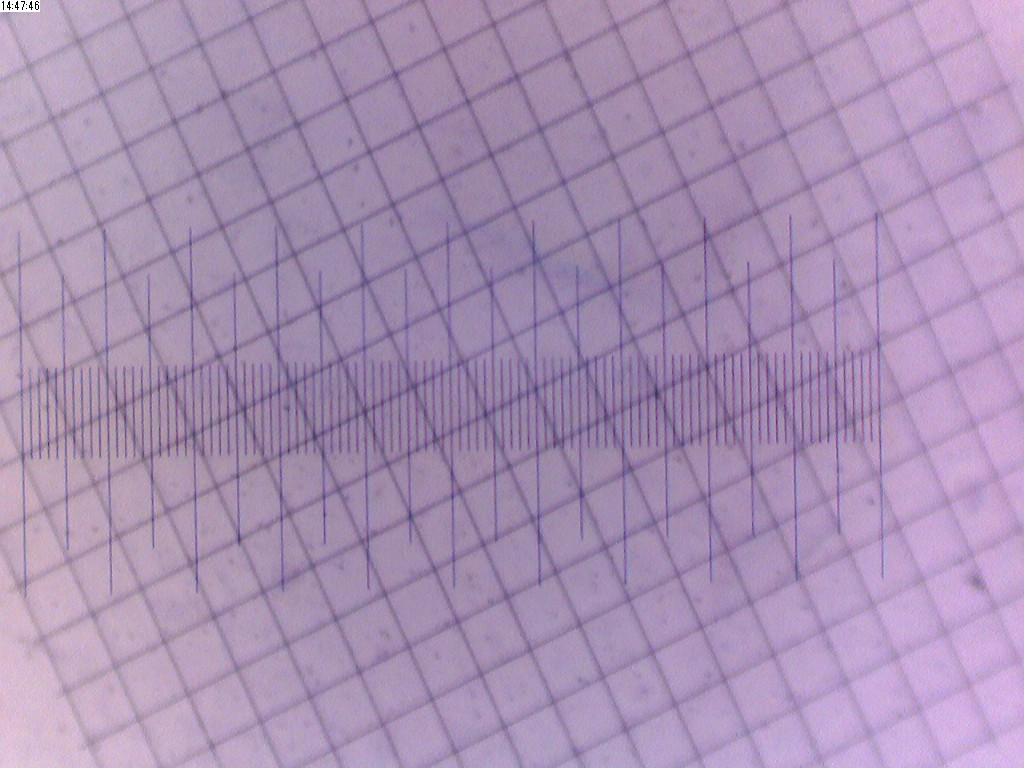
\includegraphics[width=\linewidth]{src/figures/result/meaure_slit.jpg}
        \subcaption{定規}\label{subfig:measure}
    \end{subfigure}
    \caption{スリットの画像}\label{fig:slit_image}
\end{figure}


\subsubsection{回折強度パターンの推定}
\ref{subsubsec:slit_shape}節で計測したスリットの形状をもとに、回折強度パターンを推定した。
単スリットの場合、光の透過率 \( f(x) \) は簡単のために一次元として
\begin{equation}
	f(x) =
	\begin{cases}
		1 & \text{if } |x| < a \\
		0 & \text{otherwise}
	\end{cases}
\end{equation}
と表されるから、このフーリエ変換は
\begin{equation}\label{eq:single_slit_ft}
	\begin{aligned}
		F(k) & = \int_{-\infty}^{\infty} f(x) e^{- 2 \pi i k x } \odif{x}           \\
		     & = \int_{-a}^{a} e^{- 2\pi i k x} \odif{x}                            \\
		     & = 2a \cdot \mathrm{sinc} \left( 2\pi a k \right)                     \\
		     & = 2a \cdot \mathrm{sinc} \left( \dfrac{2\pi a}{\lambda b} k  \right)
	\end{aligned}
\end{equation}
と表される。なお、 \( k \) を \( \dfrac{k}{\lambda b}  \)  と置換した。
\footnote{
	\( k \) を \( \frac{k}{\lambda b}  \)と置換するのはやや天下り的である。
	単スリットであれば、単スリットを無限小に分割し、点波源として考えれば図\ref{fig:single_slit_amp_explain}で、
	\( r_n(\epsilon) = \sqrt{b^2+ \left( x - \epsilon \right)^2} \approx \left( b + \frac{x^2}{2b} - \frac{x \epsilon}{b}   \right) \) より、
	スクリーン上の位置\( x \) における振幅 \( A(x) \) は、
	\begin{equation}
		\begin{aligned}
			A(x) & = \int_{-\frac{a}{2}}^{\frac{a}{2}} \dfrac{A_0}{a} \exp \left\{ i \dfrac{2\pi}{\lambda} \left( x - r_n(\epsilon) \right)  \right\} \odif{\epsilon}                                                       \\
			     & = \exp \left[ i \dfrac{2\pi}{\lambda} \left( b + \dfrac{x^2}{2b}  \right)  \right] \int_{-\frac{a}{2}}^{\frac{a}{2}} \exp \left[ -i \dfrac{2\pi}{\lambda} \dfrac{x \epsilon}{b}  \right] \odif{\epsilon}
		\end{aligned}
	\end{equation}
	となる。したがって、強度 \( I(x) \) は、
	\begin{equation}
		\begin{aligned}
			I(x) & = | A(x) |^2                                                                                                                            \\
			     & = \left| \int_{-\frac{a}{2}}^{\frac{a}{2}} \exp \left[ i \dfrac{2\pi}{\lambda} \dfrac{x \epsilon}{b}  \right] \odif{\epsilon} \right|^2 \\
			     & = \left| a \cdot \mathrm{sinc}\left( \dfrac{\pi a}{\lambda b} x  \right)  \right|^2
		\end{aligned}
	\end{equation}
	となり、この式で、 \( a = 2a \), \( x = k \) と置換すると、先の式が得られる。
}
また、2重スリットの場合、光の透過率 \( f(x) \) は スリットの幅を \( 2a \) 、スリットの中心座標を \( \pm x_0 \) として
\begin{equation}
	f(x) =
	\begin{cases}
		1 & \text{if } |x - x_0| < a \\
		0 & \text{otherwise}
	\end{cases}
\end{equation}
とかけるから、このフーリエ変換はフーリエ変換の性質\( \mathcal{F}[f(x-x_0)] = F(k)\exp \left( -i 2 \pi x_0 k \right) \)を用いて、
\begin{equation}\label{eq:double_slit_ft}
	\begin{aligned}
		F(k) & = 2a \cdot \mathrm{sinc} \left( \dfrac{2\pi a}{\lambda b} k  \right) \exp \left( -i \dfrac{2 \pi x_0}{\lambda b}  k \right) + 2a \cdot \mathrm{sinc} \left( \dfrac{2\pi a}{\lambda b} k  \right) \exp \left( i \dfrac{2 \pi x_0}{\lambda b}  k \right) \\
		     & = 4a \cos \left( \dfrac{2 \pi x_0}{\lambda b} k \right) \cdot \mathrm{sinc} \left( \dfrac{2\pi a}{\lambda b} k  \right)
	\end{aligned}
\end{equation}
となる。

したがって、単スリットの場合は、谷の間隔\( d \)は
\begin{equation}\label{eq:single_slit_d}
	d = \dfrac{\lambda b}{2a}
\end{equation}
となる。
また、二重スリットの場合、 \( \cos  \) の項が \( 0 \) になる場合と、 \( \mathrm{sinc}  \) の項が0になる場合がある。
前者による谷の間隔 \( d_1 \) と、後者による谷の間隔 \( d_2 \) は、
\begin{equation}\label{eq:double_slit_d}
	\begin{aligned}
		d_1 & = \dfrac{\lambda b}{2x_0} \\
		d_2 & = \dfrac{\lambda b}{2a}
	\end{aligned}
\end{equation}
となる。
一般には\( x_0 > a \) であるから、大きいなうねりが単スリットと同様に \( \mathrm{sinc} \) の項により生じ、小さいなうねりが \( \cos \) の項により生じる。


コンピュータを用いて円スリット、単スリット、2重スリットに対して、2次元のフーリエ変換を計算し、回折強度パターンをシミュレーションした結果を図\ref{fig:amplitude_sim_circle}、図\ref{fig:amplitude_sim_single}、図\ref{fig:amplitude_sim_dual}に示す。

\begin{figure}[htbp]
	\centering
	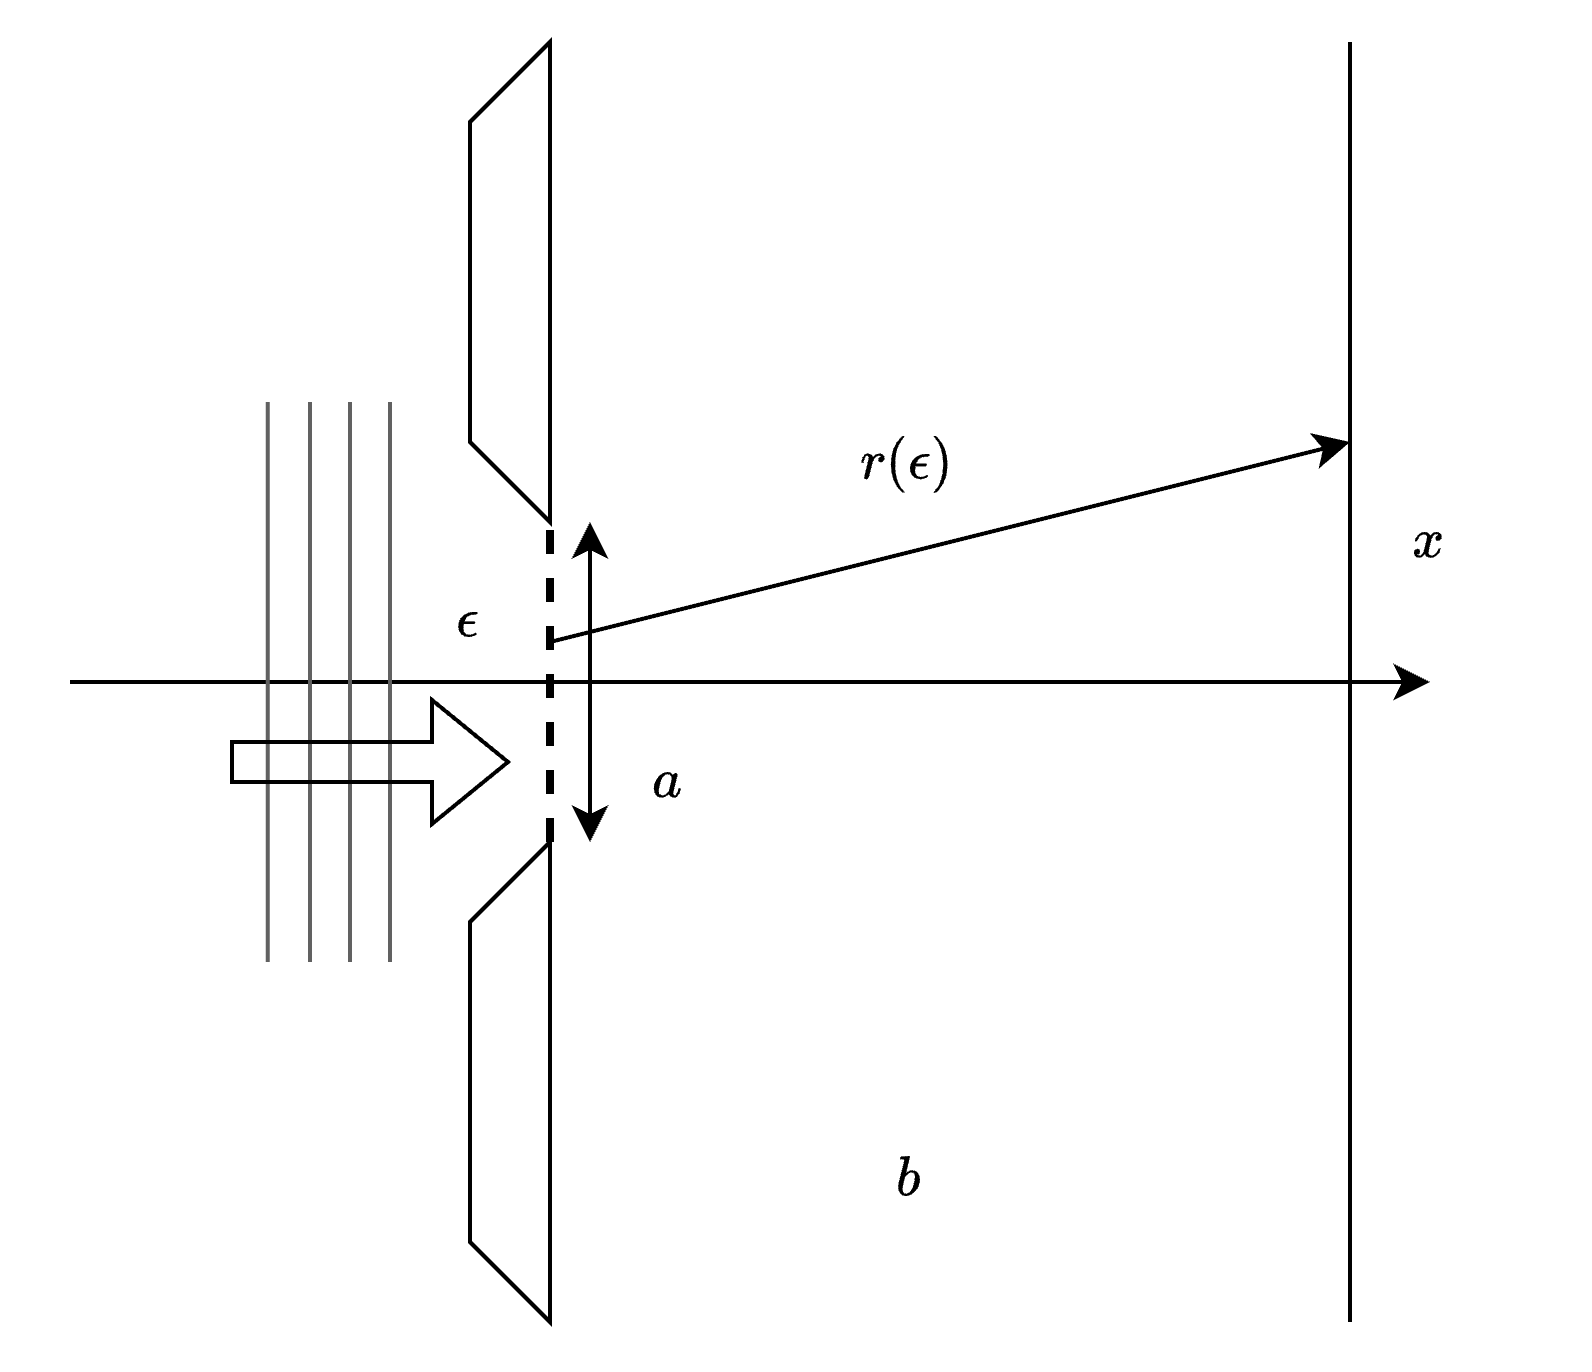
\includegraphics[width=0.5\linewidth]{src/figures/result/signle_slit_amp_explain.png}
	\caption{単スリット回折強度}
	\label{fig:single_slit_amp_explain}
\end{figure}

\begin{figure}[htbp]
	\begin{minipage}[ht]{0.48\hsize}\centering
		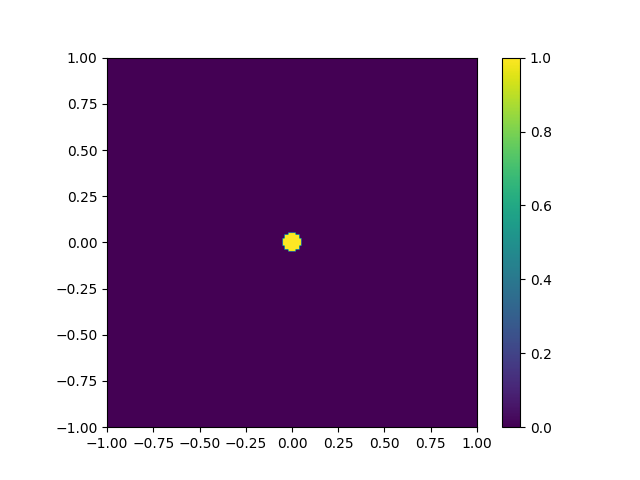
\includegraphics[width=\linewidth]{src/figures/result/circle1_original_estimation.png}
		\subcaption{円スリット (半径0.05)}\label{subfig:amplitude_sim_circle1_original}
	\end{minipage}
	\begin{minipage}[ht]{0.48\hsize}\centering
		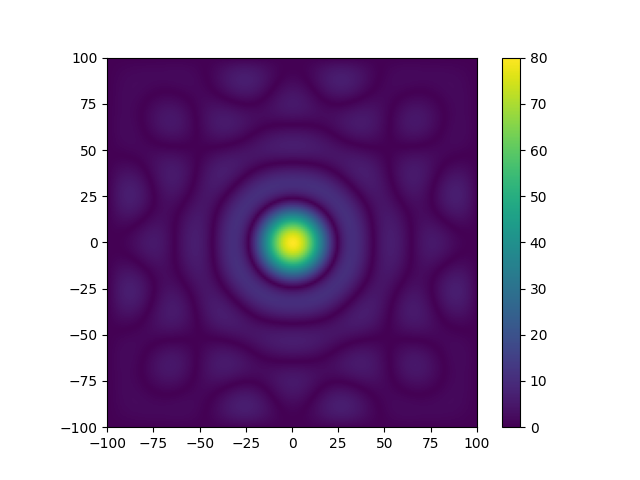
\includegraphics[width=\linewidth]{src/figures/result/circle1_amplitude_estimation.png}
		\subcaption{円スリット (半径0.05)の回折強度パターン}\label{subfig:amplitude_sim_circle1}
	\end{minipage}

	\begin{minipage}[ht]{0.48\hsize}\centering
		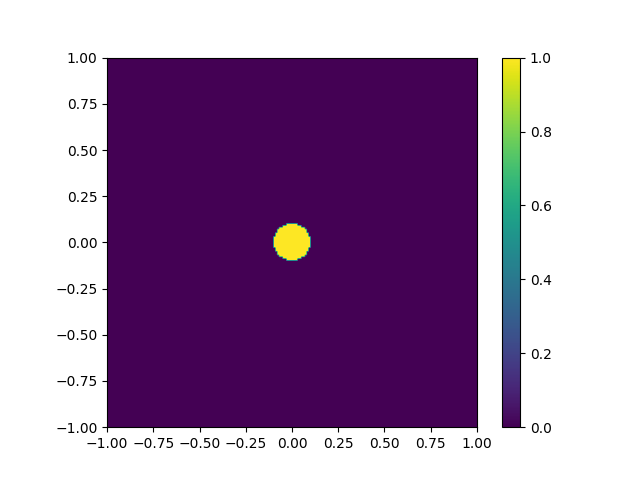
\includegraphics[width=\linewidth]{src/figures/result/circle2_original_estimation.png}
		\subcaption{円スリット (半径0.1)}\label{subfig:amplitude_sim_circle2_original}
	\end{minipage}
	\begin{minipage}[ht]{0.48\hsize}\centering
		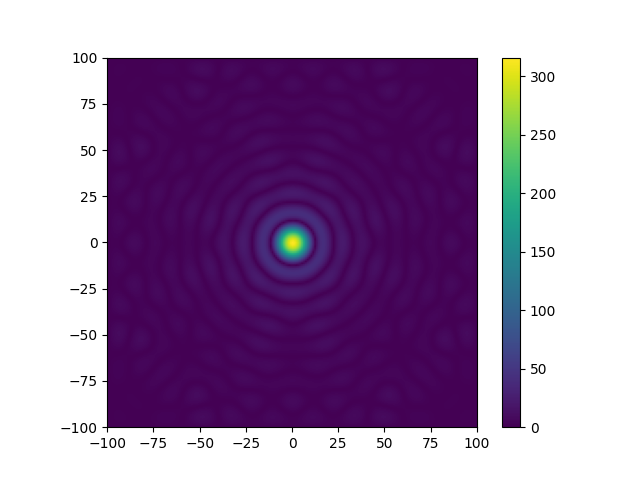
\includegraphics[width=\linewidth]{src/figures/result/circle2_amplitude_estimation.png}
		\subcaption{円スリット (半径0.1)の回折強度パターン}\label{subfig:amplitude_sim_circle2}
	\end{minipage}
	\caption{円スリットの回折強度パターンのシミュレーション}\label{fig:amplitude_sim_circle}
\end{figure}

\begin{figure}[htbp]
	\begin{minipage}[ht]{0.48\hsize}\centering
		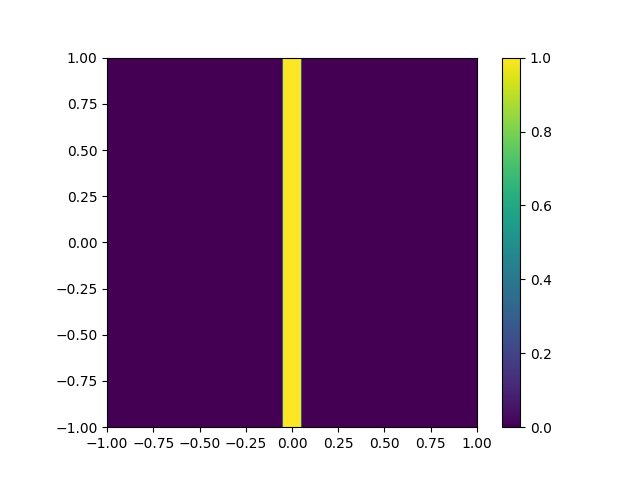
\includegraphics[width=\linewidth]{src/figures/result/ss1_original_estimation.png}
		\subcaption{単スリット (幅 0.05)}\label{subfig:amplitude_sim_single1_original}
	\end{minipage}
	\begin{minipage}[ht]{0.48\hsize}\centering
		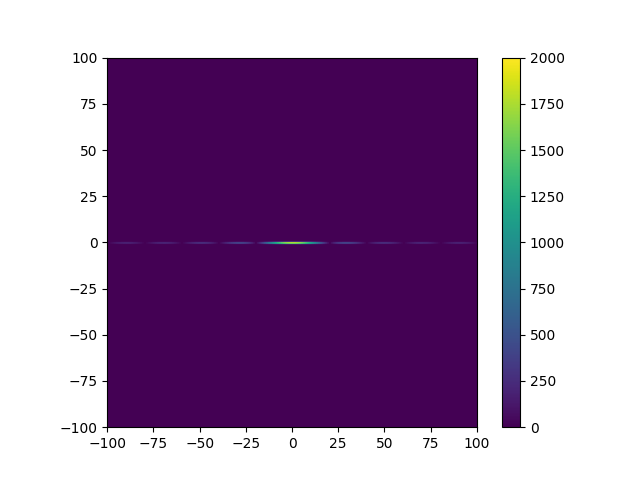
\includegraphics[width=\linewidth]{src/figures/result/ss1_amplitude_estimation.png}
		\subcaption{単スリット (幅 0.05)の回折強度パターン}\label{subfig:amplitude_sim_single1}
	\end{minipage}
	\begin{minipage}[ht]{0.48\hsize}\centering
		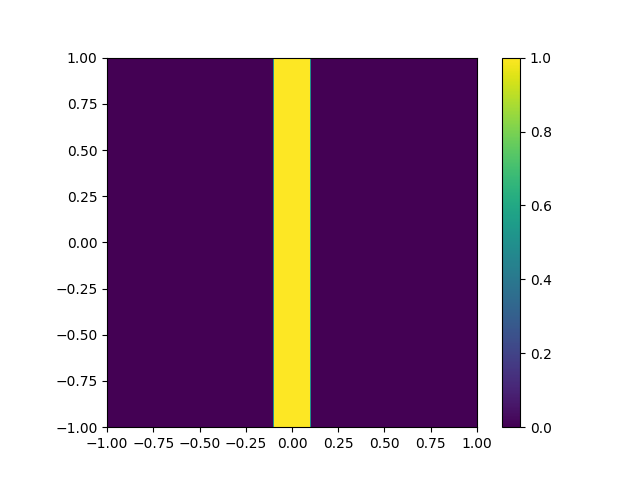
\includegraphics[width=\linewidth]{src/figures/result/ss2_original_estimation.png}
		\subcaption{単スリット (幅 0.1)}\label{subfig:amplitude_sim_single2_original}
	\end{minipage}
	\begin{minipage}[ht]{0.48\hsize}\centering
		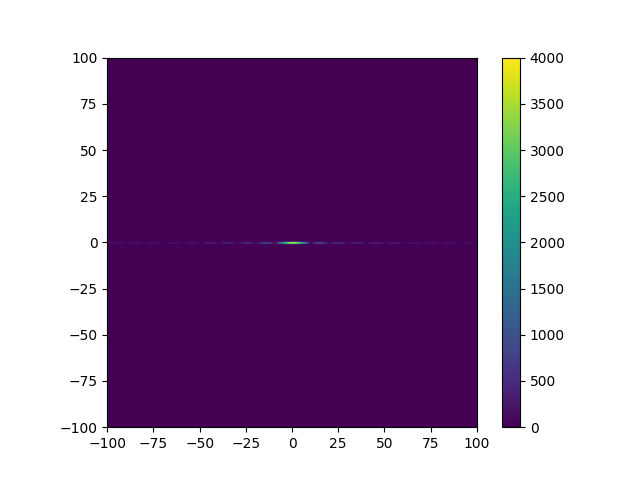
\includegraphics[width=\linewidth]{src/figures/result/ss2_amplitude_estimation.png}
		\subcaption{単スリット (幅 0.1)の回折強度パターン}\label{subfig:amplitude_sim_single2}
	\end{minipage}
	\caption{単スリットの回折強度パターンのシミュレーション}\label{fig:amplitude_sim_single}
\end{figure}

\begin{figure}[htbp]
	\begin{minipage}[ht]{0.48\hsize}\centering
		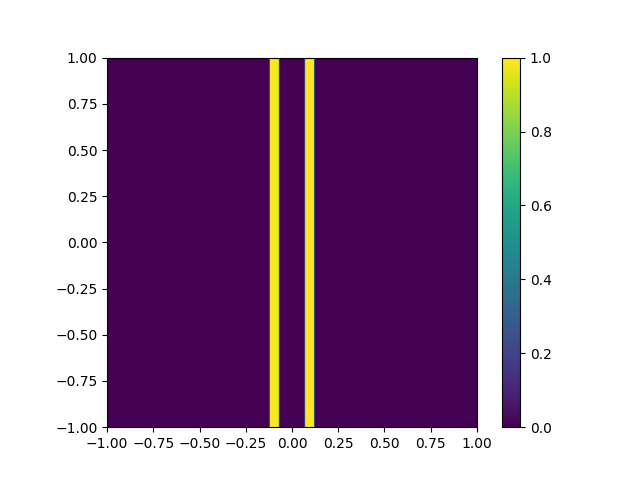
\includegraphics[width=\linewidth]{src/figures/result/ds1_original_estimation.png}
		\subcaption{二重スリット (幅 0.05, 間隔 0.1)}\label{subfig:amplitude_sim_dual1_original}
	\end{minipage}
	\begin{minipage}[ht]{0.48\hsize}\centering
		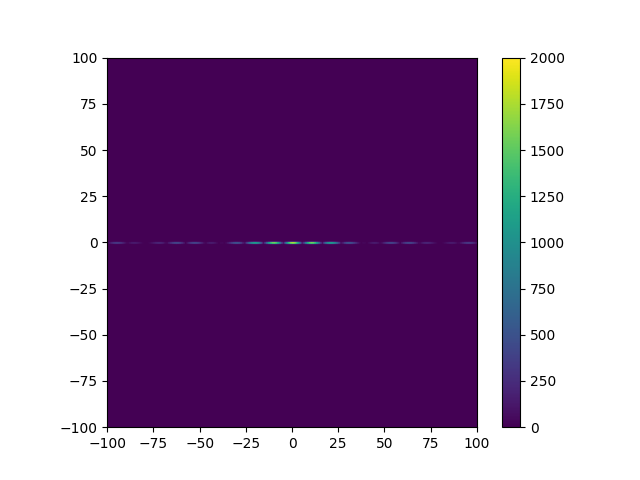
\includegraphics[width=\linewidth]{src/figures/result/ds1_amplitude_estimation.png}
		\subcaption{二重スリット (幅 0.05, 間隔 0.1)の回折強度パターン}\label{subfig:amplitude_sim_dual1}
	\end{minipage}
	\begin{minipage}[ht]{0.48\hsize}\centering
		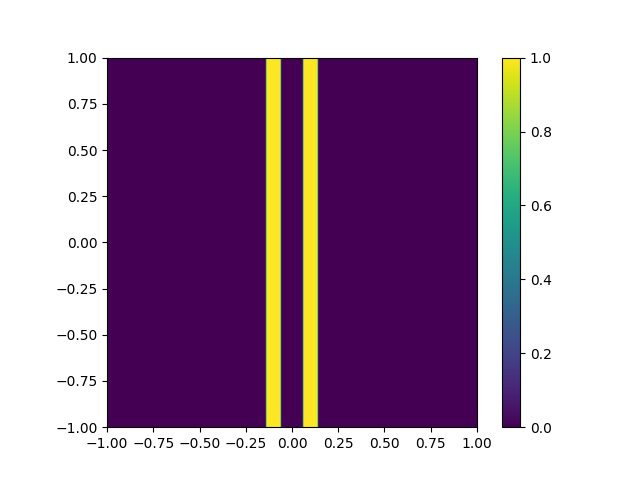
\includegraphics[width=\linewidth]{src/figures/result/ds2_original_estimation.png}
		\subcaption{二重スリット (幅 0.08, 間隔 0.1)}\label{subfig:amplitude_sim_dual2_original}
	\end{minipage}
	\begin{minipage}[ht]{0.48\hsize}\centering
		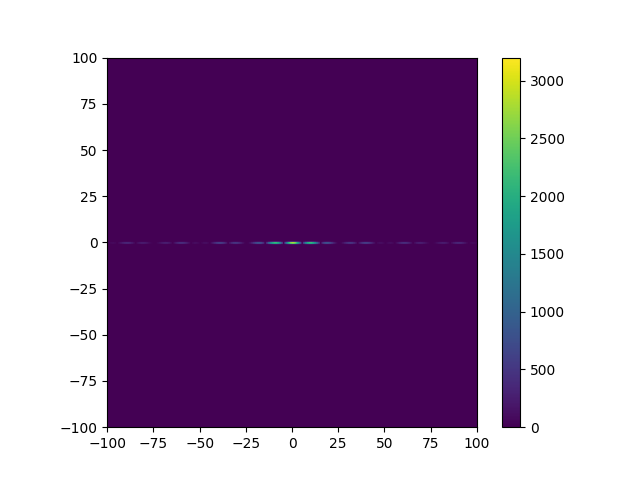
\includegraphics[width=\linewidth]{src/figures/result/ds2_amplitude_estimation.png}
		\subcaption{二重スリット (幅 0.08, 間隔 0.1)の回折強度パターン}\label{subfig:amplitude_sim_dual2}
	\end{minipage}
	\begin{minipage}[ht]{0.48\hsize}\centering
		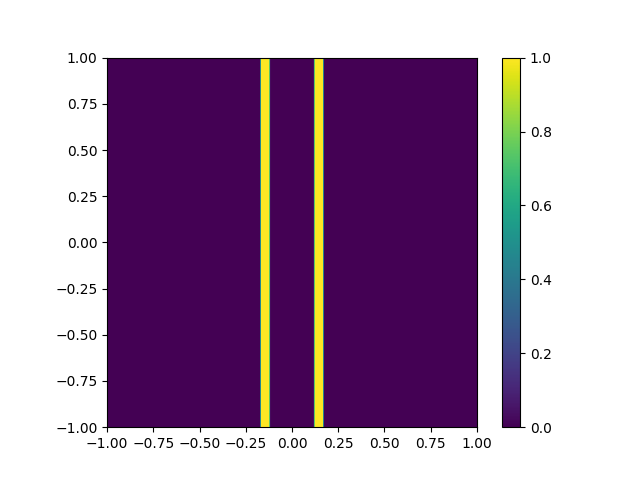
\includegraphics[width=\linewidth]{src/figures/result/ds3_original_estimation.png}
		\subcaption{二重スリット (幅 0.05, 間隔 0.15)}\label{subfig:amplitude_sim_dual3_original}
	\end{minipage}
	\begin{minipage}[ht]{0.48\hsize}\centering
		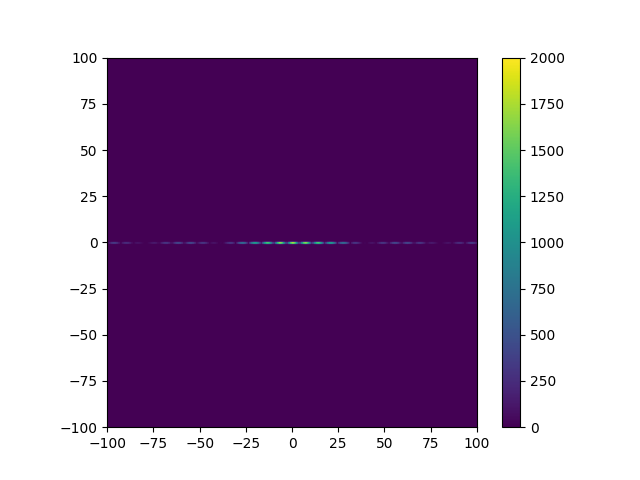
\includegraphics[width=\linewidth]{src/figures/result/ds3_amplitude_estimation.png}
		\subcaption{二重スリット (幅 0.05, 間隔 0.15)の回折強度パターン}\label{subfig:amplitude_sim_dual3}
	\end{minipage}
	\caption{単スリットの回折強度パターンのシミュレーション}\label{fig:amplitude_sim_dual}
\end{figure}


\subsubsection{回折強度パターンの測定結果}
実際に使用したレーザーの波長は \SI{632.8}{\nano\meter} 、開口とスクリーンの距離は \SI{96.5}{cm}であった。
このときに、\ref{subsubsec:slit_shape}節で計測したスリットに対してレーザーを照射し、スクリーンに写った像を撮影した。
その結果を図\ref{fig:screen_photo}に示す。
図\ref{subfig:screen_measure}は、画像のピクセルと実際の大きさを対応させるために \SI{15}{cm} の定規をおいて撮影したものである。
この画像から、\SI{193.00}{pixel}が\SI{3.00}{cm}すなわち、\SI{0.0155}{cm/pixel}であると計算された。
これをもとに、画像のグレースケールを強度として取り出し、実際の大きさに変換したものを図\ref{fig:amplitude}に示す。
グレースケールは最大値を1として正規化されている。


単スリット・二重スリットの回折強度パターンの谷の間隔は、式\ref{eq:single_slit_d}、式\ref{eq:double_slit_d}から
表\ref{tab:ss_slit_width}、表\ref{tab:ds_slit_width}のようになった。
計測値は\ref{subsubsec:slit_shape}で測定されたもの、計算値が上記の式から計算された値である。

%Please add the following packages if necessary:
%\usepackage{booktabs, multirow} % for borders and merged ranges
%\usepackage{soul}% for underlines
%\usepackage{xcolor,colortbl} % for cell colors
%\usepackage{changepage,threeparttable} % for wide tables
%If the table is too wide, replace \begin{table}[!htp]...\end{table} with
%\begin{adjustwidth}{-2.5 cm}{-2.5 cm}\centering\begin{threeparttable}[!htb]...\end{threeparttable}\end{adjustwidth}
\begin{table}[!htp]\centering
	\caption{単スリットのスリット幅}\label{tab:ss_slit_width}
	\scriptsize
	\begin{tabular}{ccc}\toprule
		       & 計測 / \si{\micro\meter} & 谷間隔からの計算値 / \si{\micro\meter} \\\midrule
		単スリット1 & 43.004                 & 45.858                        \\
		単スリット2 & 86.456                 & 87.952                        \\
		単スリット3 & 129.520                & 132.558                       \\
		\bottomrule
	\end{tabular}
\end{table}

%Please add the following packages if necessary:
%\usepackage{booktabs, multirow} % for borders and merged ranges
%\usepackage{soul}% for underlines
%\usepackage{xcolor,colortbl} % for cell colors
%\usepackage{changepage,threeparttable} % for wide tables
%If the table is too wide, replace \begin{table}[!htp]...\end{table} with
%\begin{adjustwidth}{-2.5 cm}{-2.5 cm}\centering\begin{threeparttable}[!htb]...\end{threeparttable}\end{adjustwidth}
\begin{table}[!htp]\centering
    \caption{二重スリットのスリット間隔と幅}\label{tab:ds_slit_width}
    \scriptsize
    \begin{tabular}{ccccc}\toprule
            & スリット幅 計測値 / \si{\micro\meter} & スリット間隔 計測値 / \si{\micro\meter} & スリット幅 計算値 / \si{\micro\meter} & スリット間隔 計算値 \si{\micro\meter} \\\midrule
        DS1 & 57.035                        & 152.41                         & 59.825                        & 180.54                       \\
        DS2 & 82.344                        & 153.49                         & 82.706                        & 197.77                       \\
        DS3 & 82.187                        & 385.86                         & 84.183                        & 448.97                       \\
        \bottomrule
    \end{tabular}
\end{table}


\begin{figure}[htbp]
	\begin{minipage}[ht]{0.48\hsize}\centering
		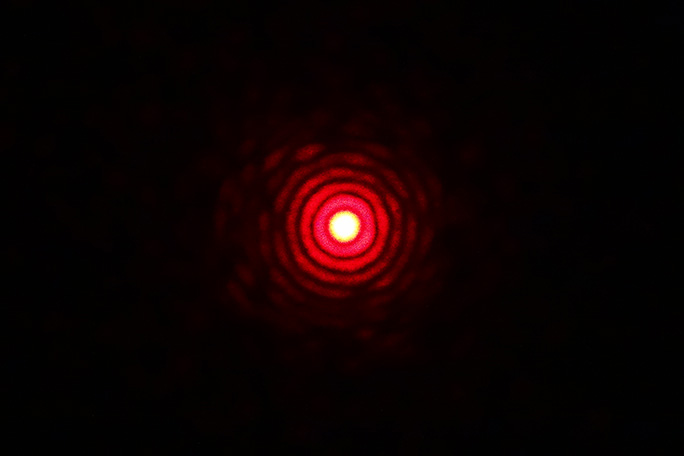
\includegraphics[width=\linewidth]{src/figures/result/CIRCLE.jpg}
		\subcaption{円スリット}\label{subfig:circle_screen}
	\end{minipage}
	\begin{minipage}[ht]{0.48\hsize}\centering
		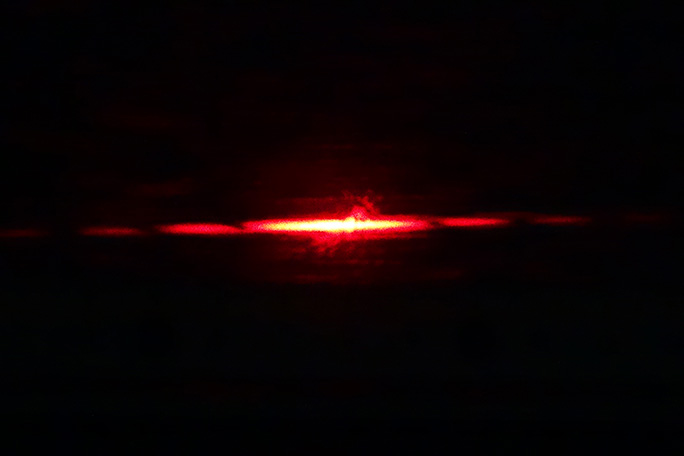
\includegraphics[width=\linewidth]{src/figures/result/SS1.JPG}
		\subcaption{単スリット1}\label{subfig:ss1_screen}
	\end{minipage}
	\begin{minipage}[ht]{0.48\hsize}\centering
		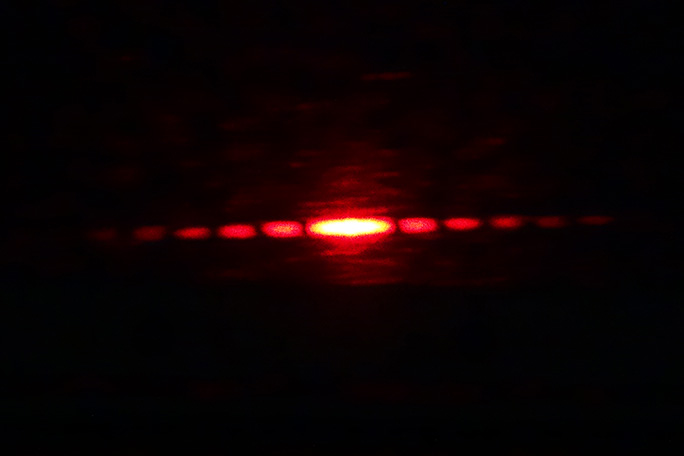
\includegraphics[width=\linewidth]{src/figures/result/SS2.JPG}
		\subcaption{単スリット2}\label{subfig:ss2_screen}
	\end{minipage}
	\begin{minipage}[ht]{0.48\hsize}\centering
		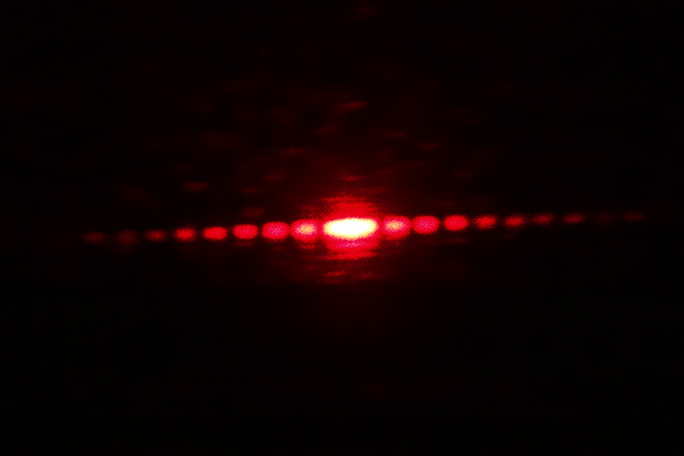
\includegraphics[width=\linewidth]{src/figures/result/SS3.JPG}
		\subcaption{単スリット3}\label{subfig:ss3_screen}
	\end{minipage}
	\begin{minipage}[ht]{0.48\hsize}\centering
		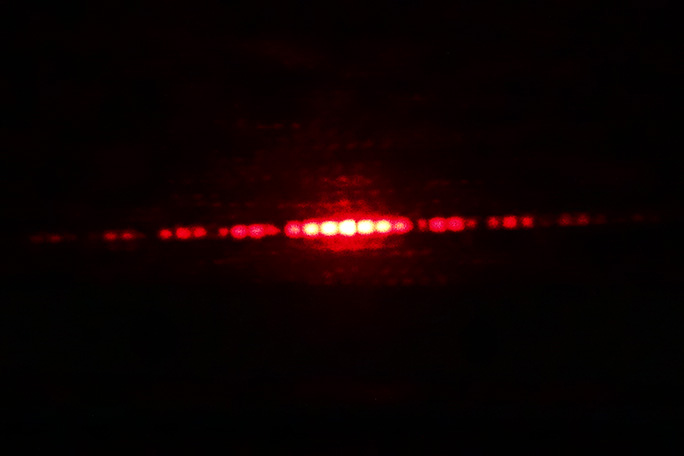
\includegraphics[width=\linewidth]{src/figures/result/DS1.JPG}
		\subcaption{ダブルスリット1}\label{subfig:ds1_screen}
	\end{minipage}
	\begin{minipage}[ht]{0.48\hsize}\centering
		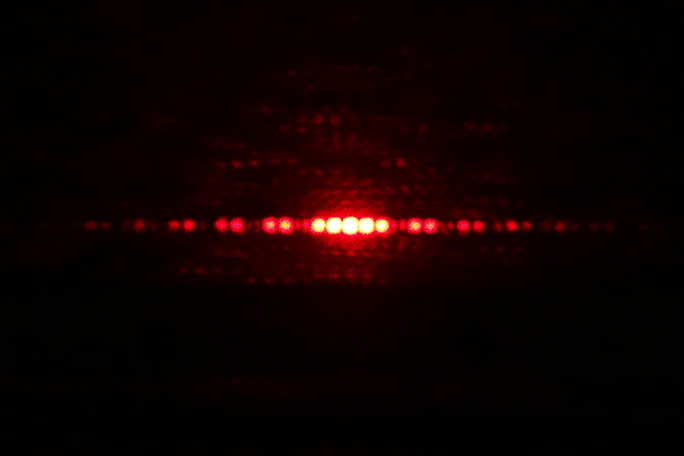
\includegraphics[width=\linewidth]{src/figures/result/DS2.JPG}
		\subcaption{ダブルスリット2}\label{subfig:ds2_screen}
	\end{minipage}
\end{figure}
\begin{figure}[htbp]
	\centering
	\addtocounter{figure}{-1}
	\begin{subfigure}{0.48\hsize}
		\addtocounter{subfigure}{6}\centering
		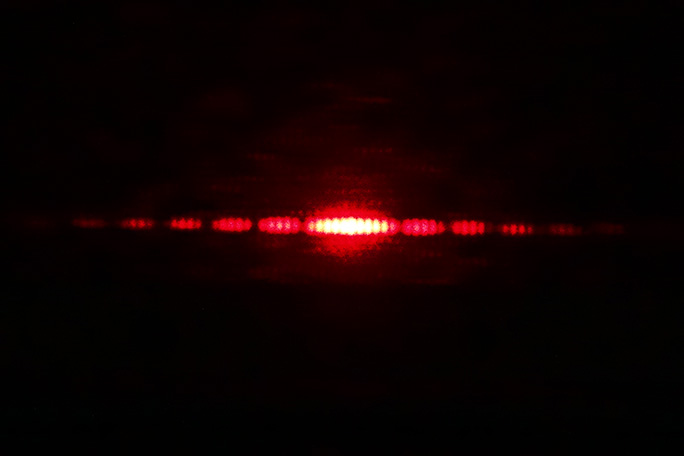
\includegraphics[width=\linewidth]{src/figures/result/DS3.JPG}
		\subcaption{ダブルスリット3}\label{subfig:ds3_screen}
	\end{subfigure}
	\begin{subfigure}{0.48\hsize}\centering
		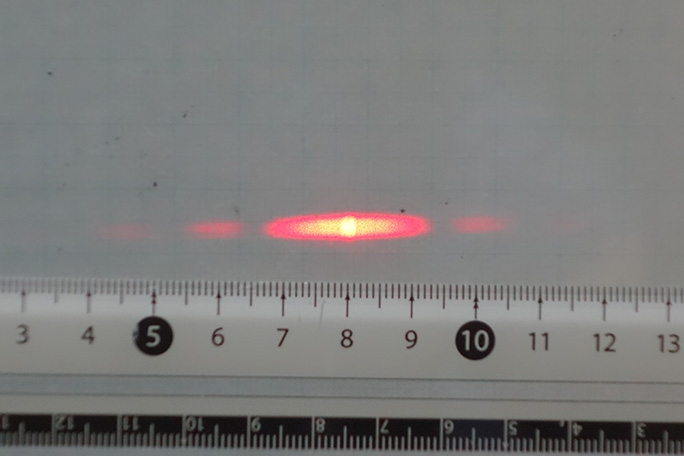
\includegraphics[width=\linewidth]{src/figures/result/measure.JPG}
		\subcaption{定規}\label{subfig:screen_measure}
	\end{subfigure}
	\caption{測定結果の写真}\label{fig:screen_photo}
\end{figure}

\begin{figure}[htbp]
	\begin{minipage}[ht]{0.48\hsize}\centering
		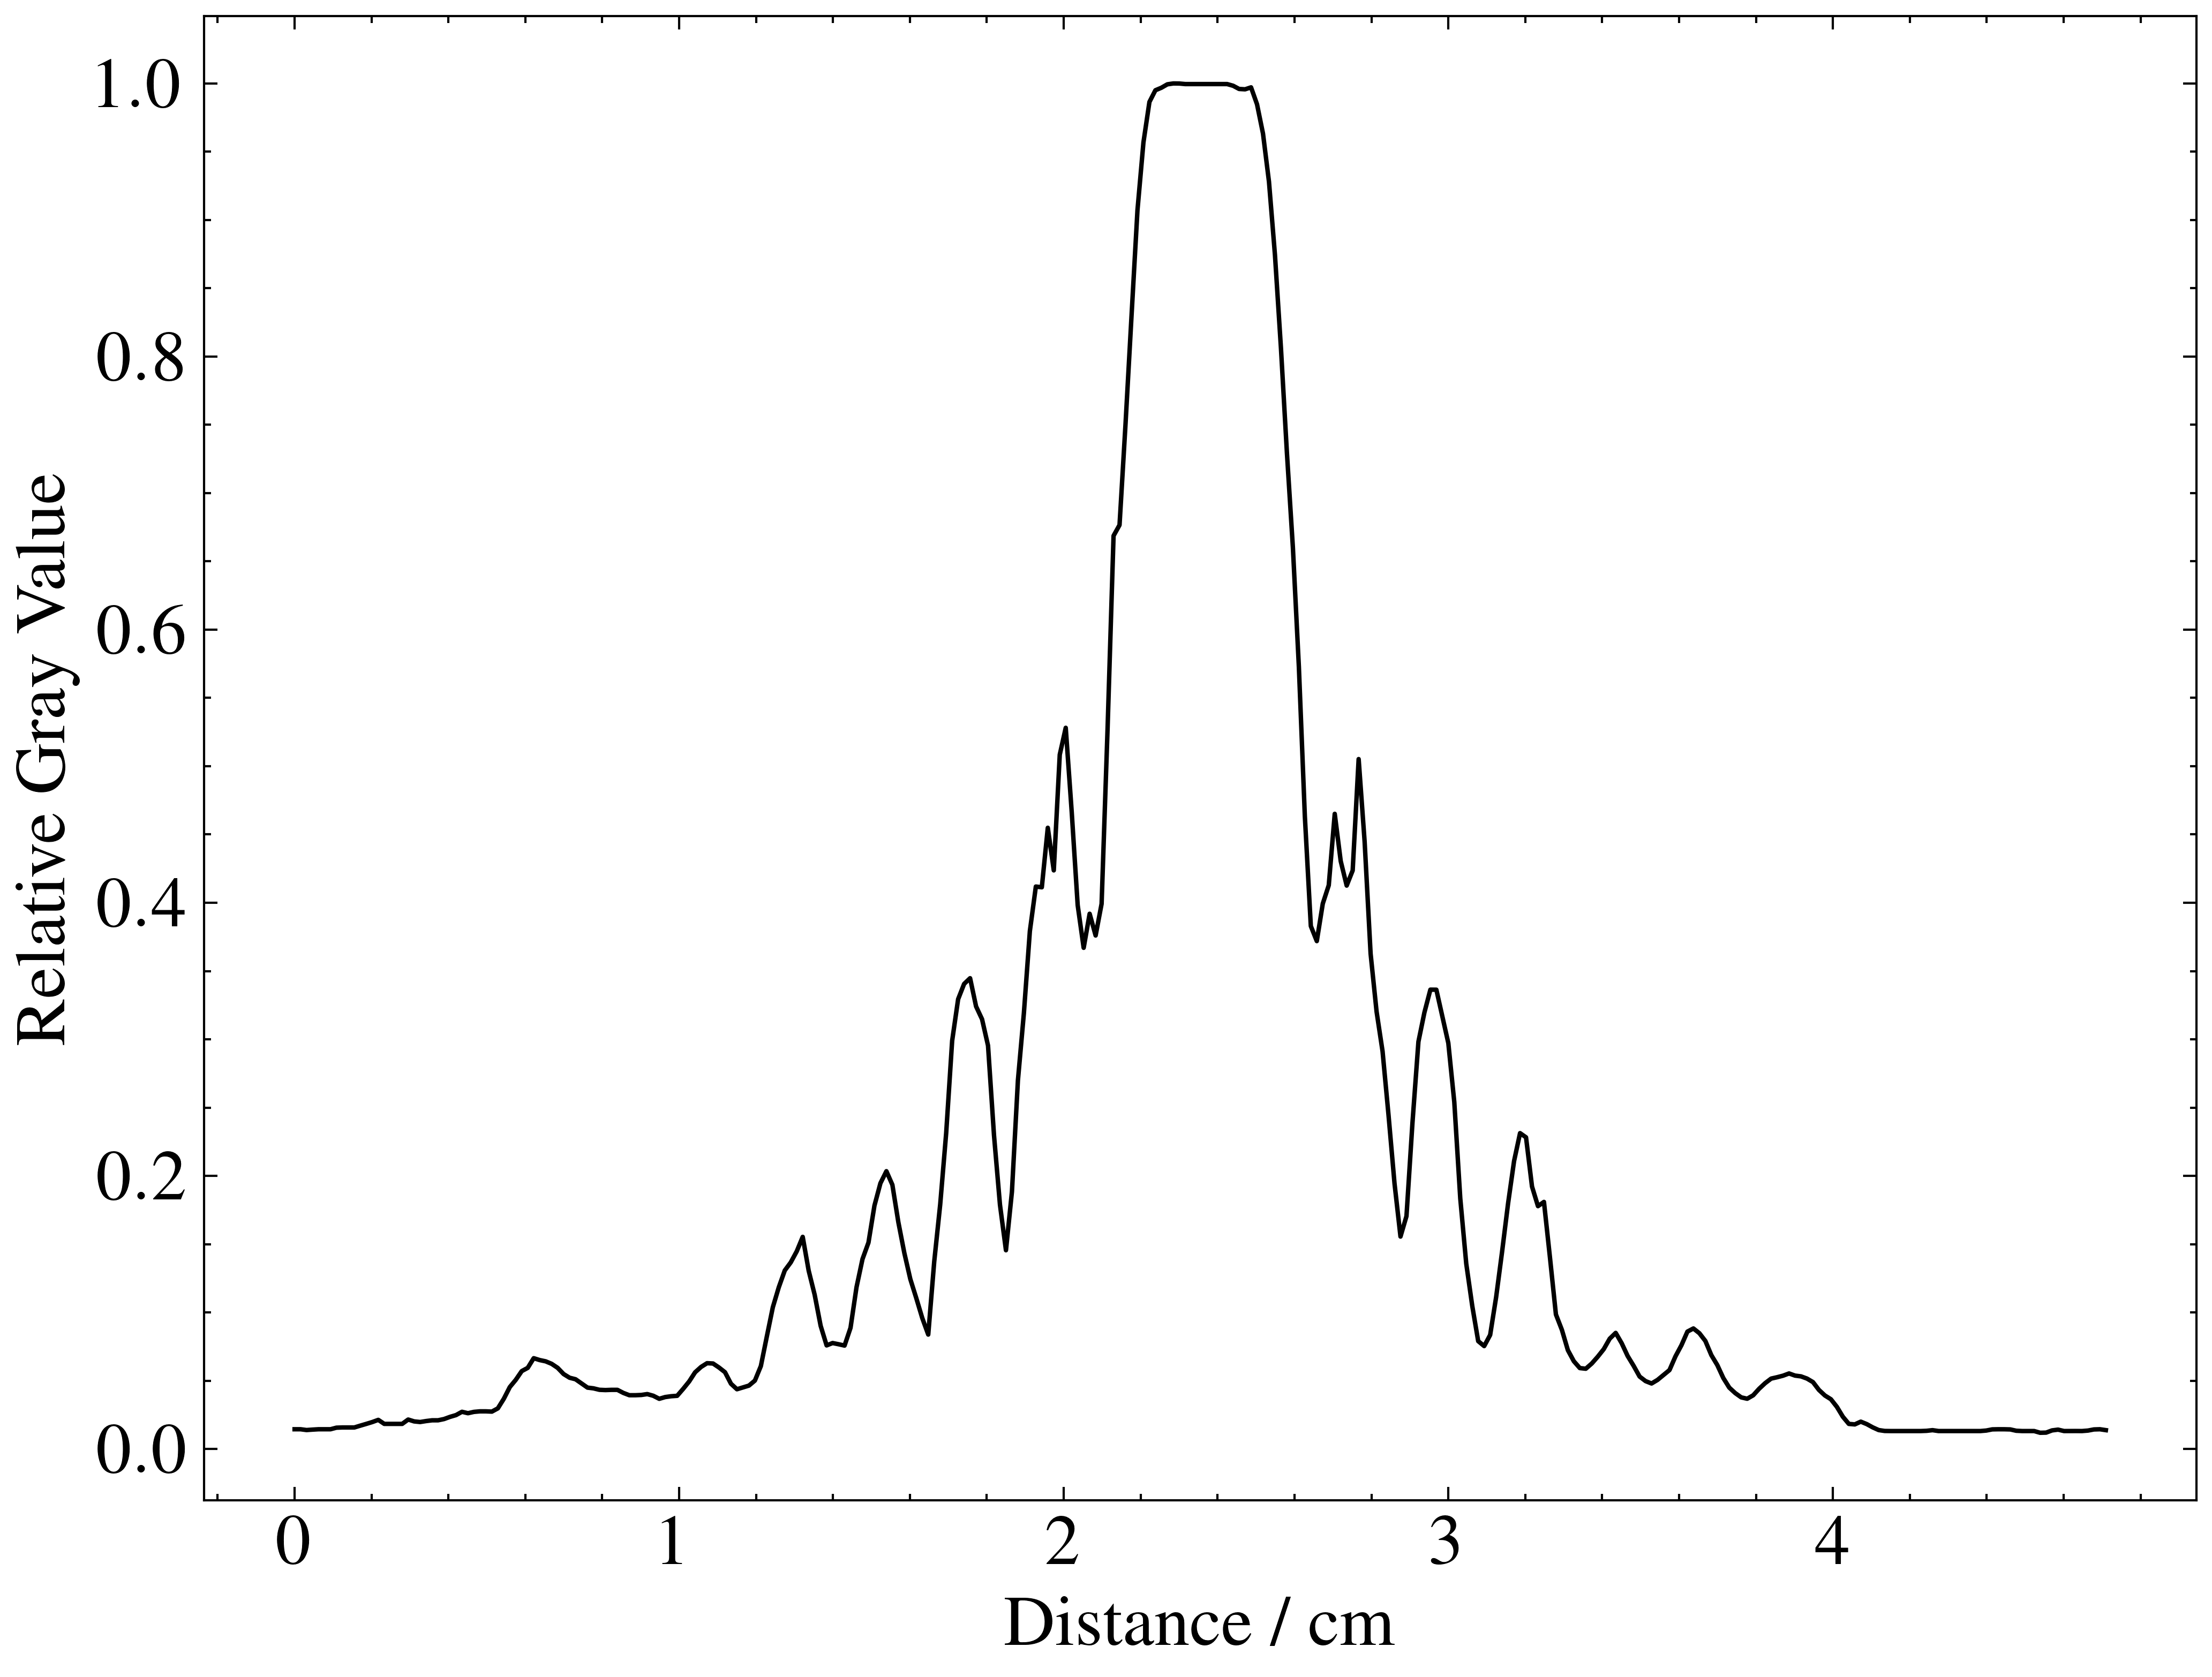
\includegraphics[width=\linewidth]{src/figures/result/circle_data_amp.png}
		\subcaption{円スリット}\label{subfig:circle_amp}
	\end{minipage}
	\begin{minipage}[ht]{0.48\hsize}\centering
		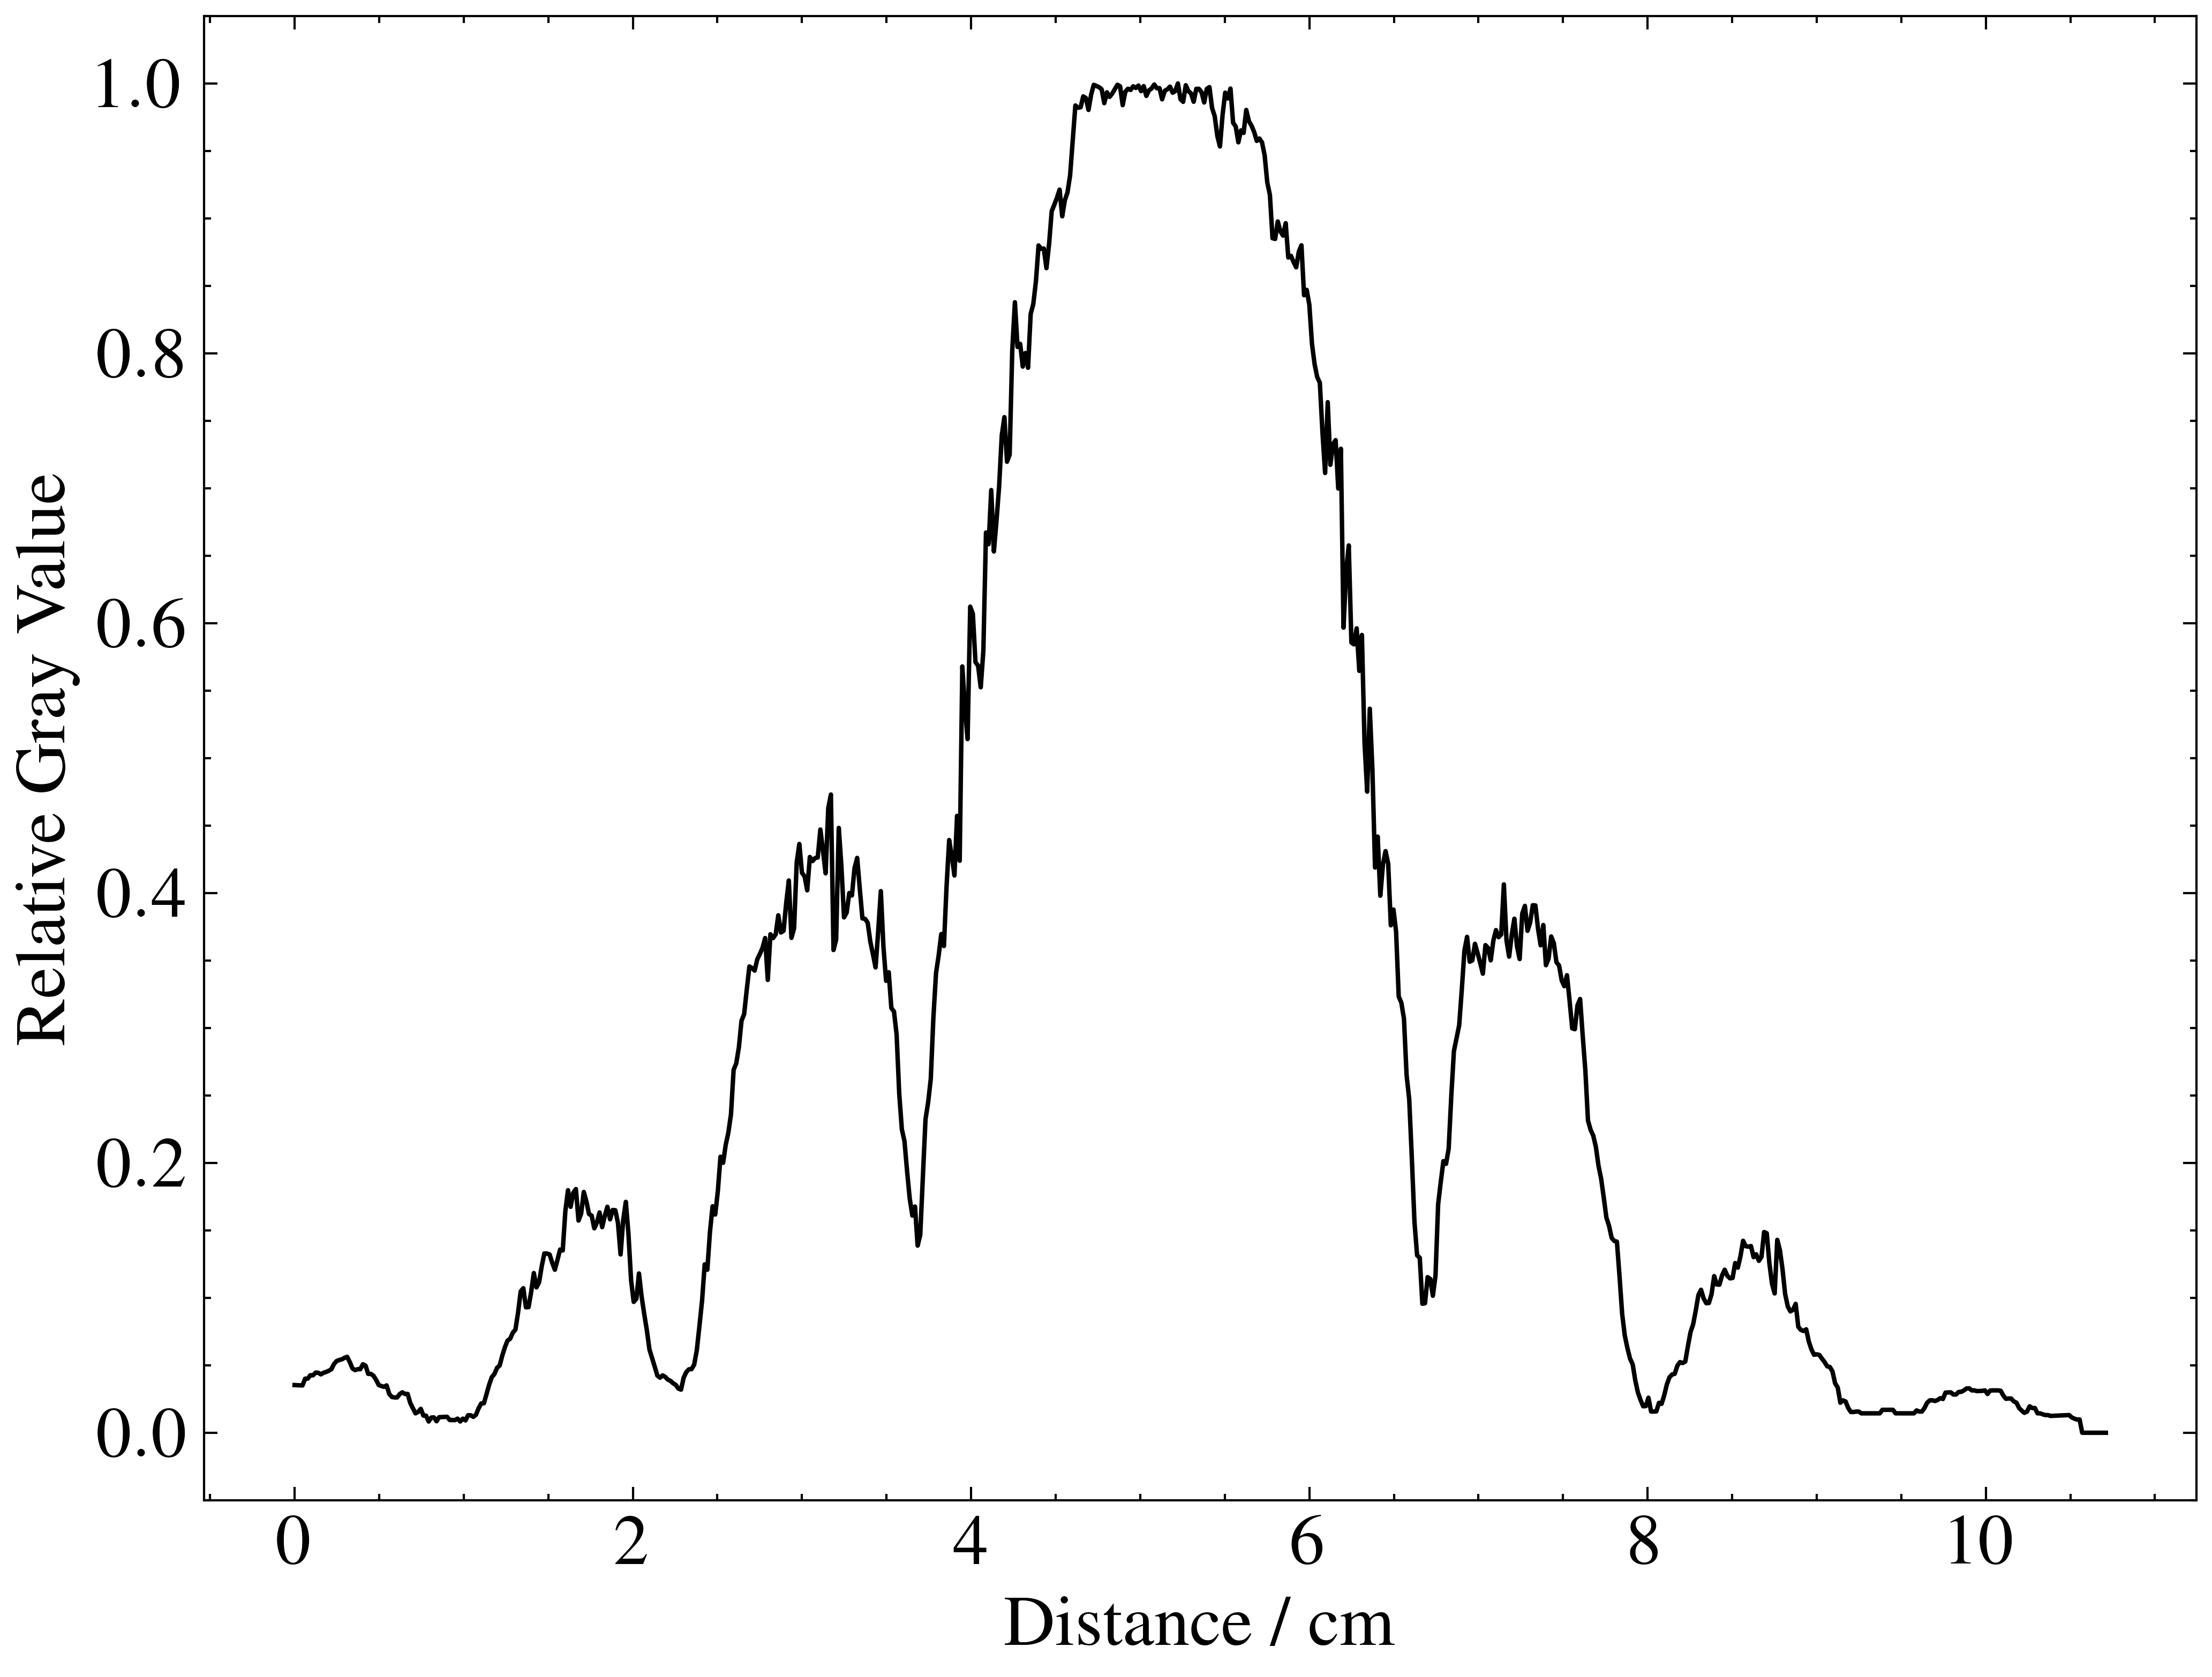
\includegraphics[width=\linewidth]{src/figures/result/ss1_data_amp.png}
		\subcaption{単スリット1}\label{subfig:ss1_amp}
	\end{minipage}
	\begin{minipage}[ht]{0.48\hsize}\centering
		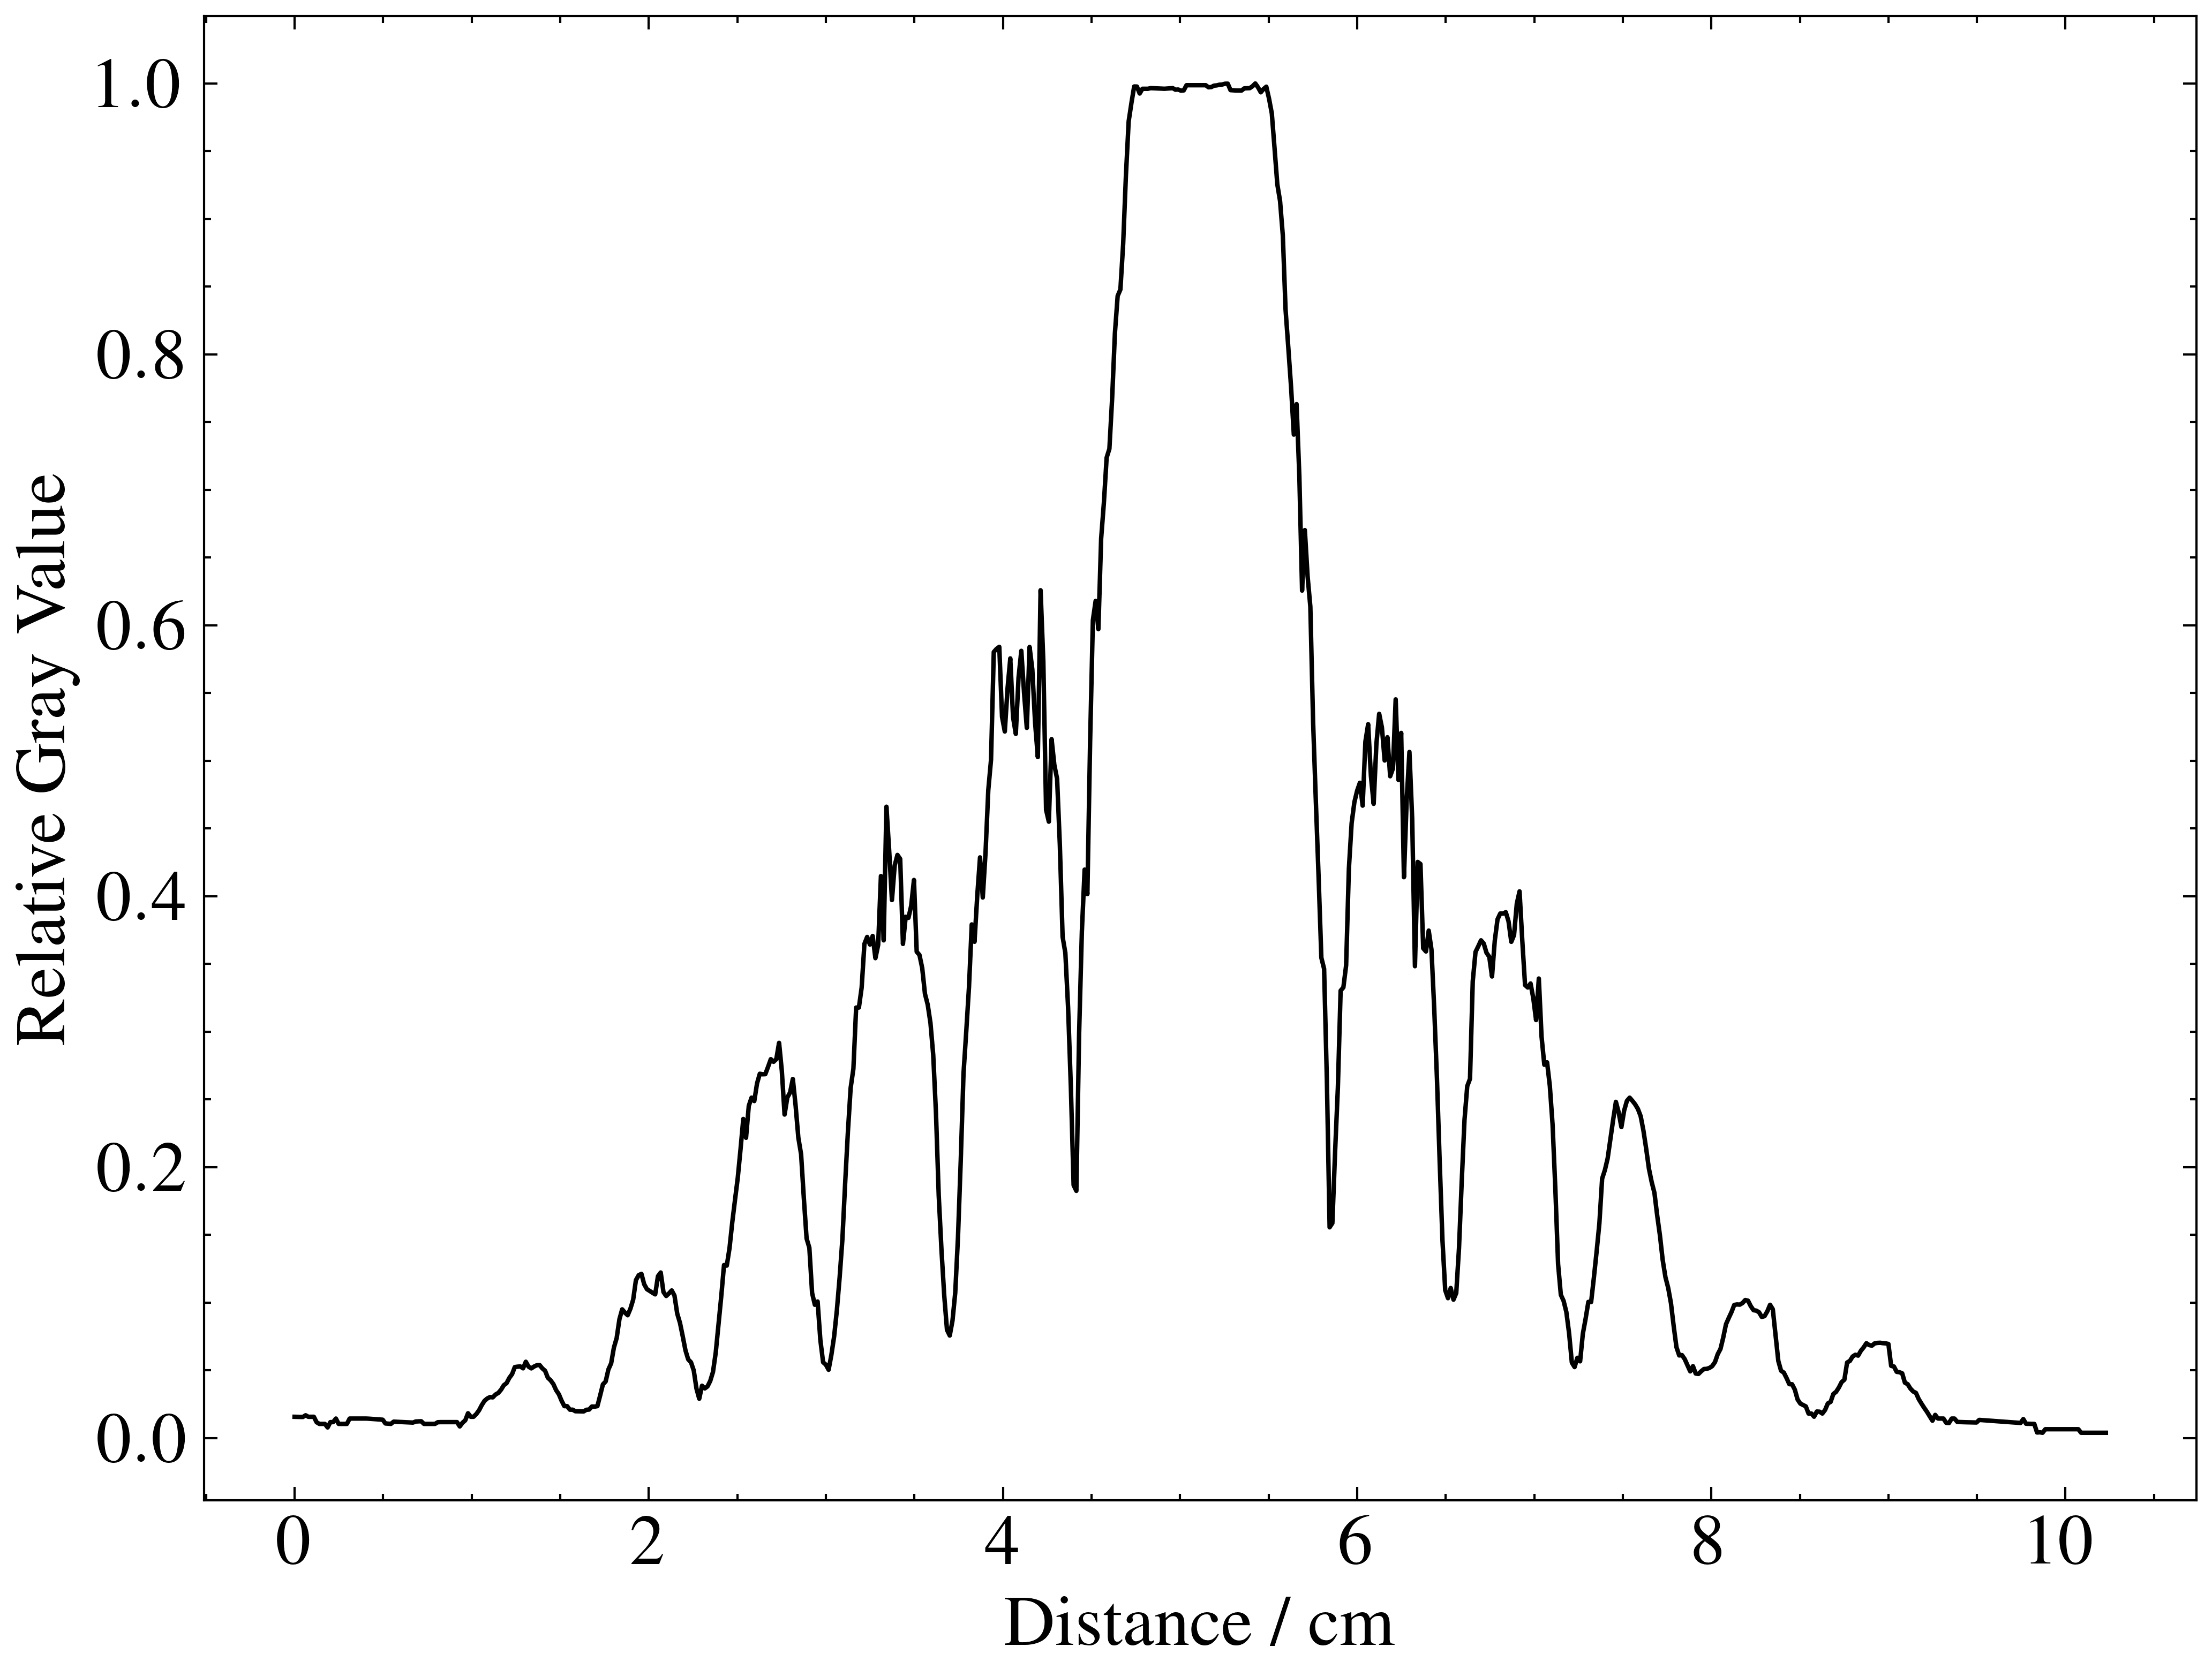
\includegraphics[width=\linewidth]{src/figures/result/ss2_data_amp.png}
		\subcaption{単スリット2}\label{subfig:ss2_amp}
	\end{minipage}
	\begin{minipage}[ht]{0.48\hsize}\centering
		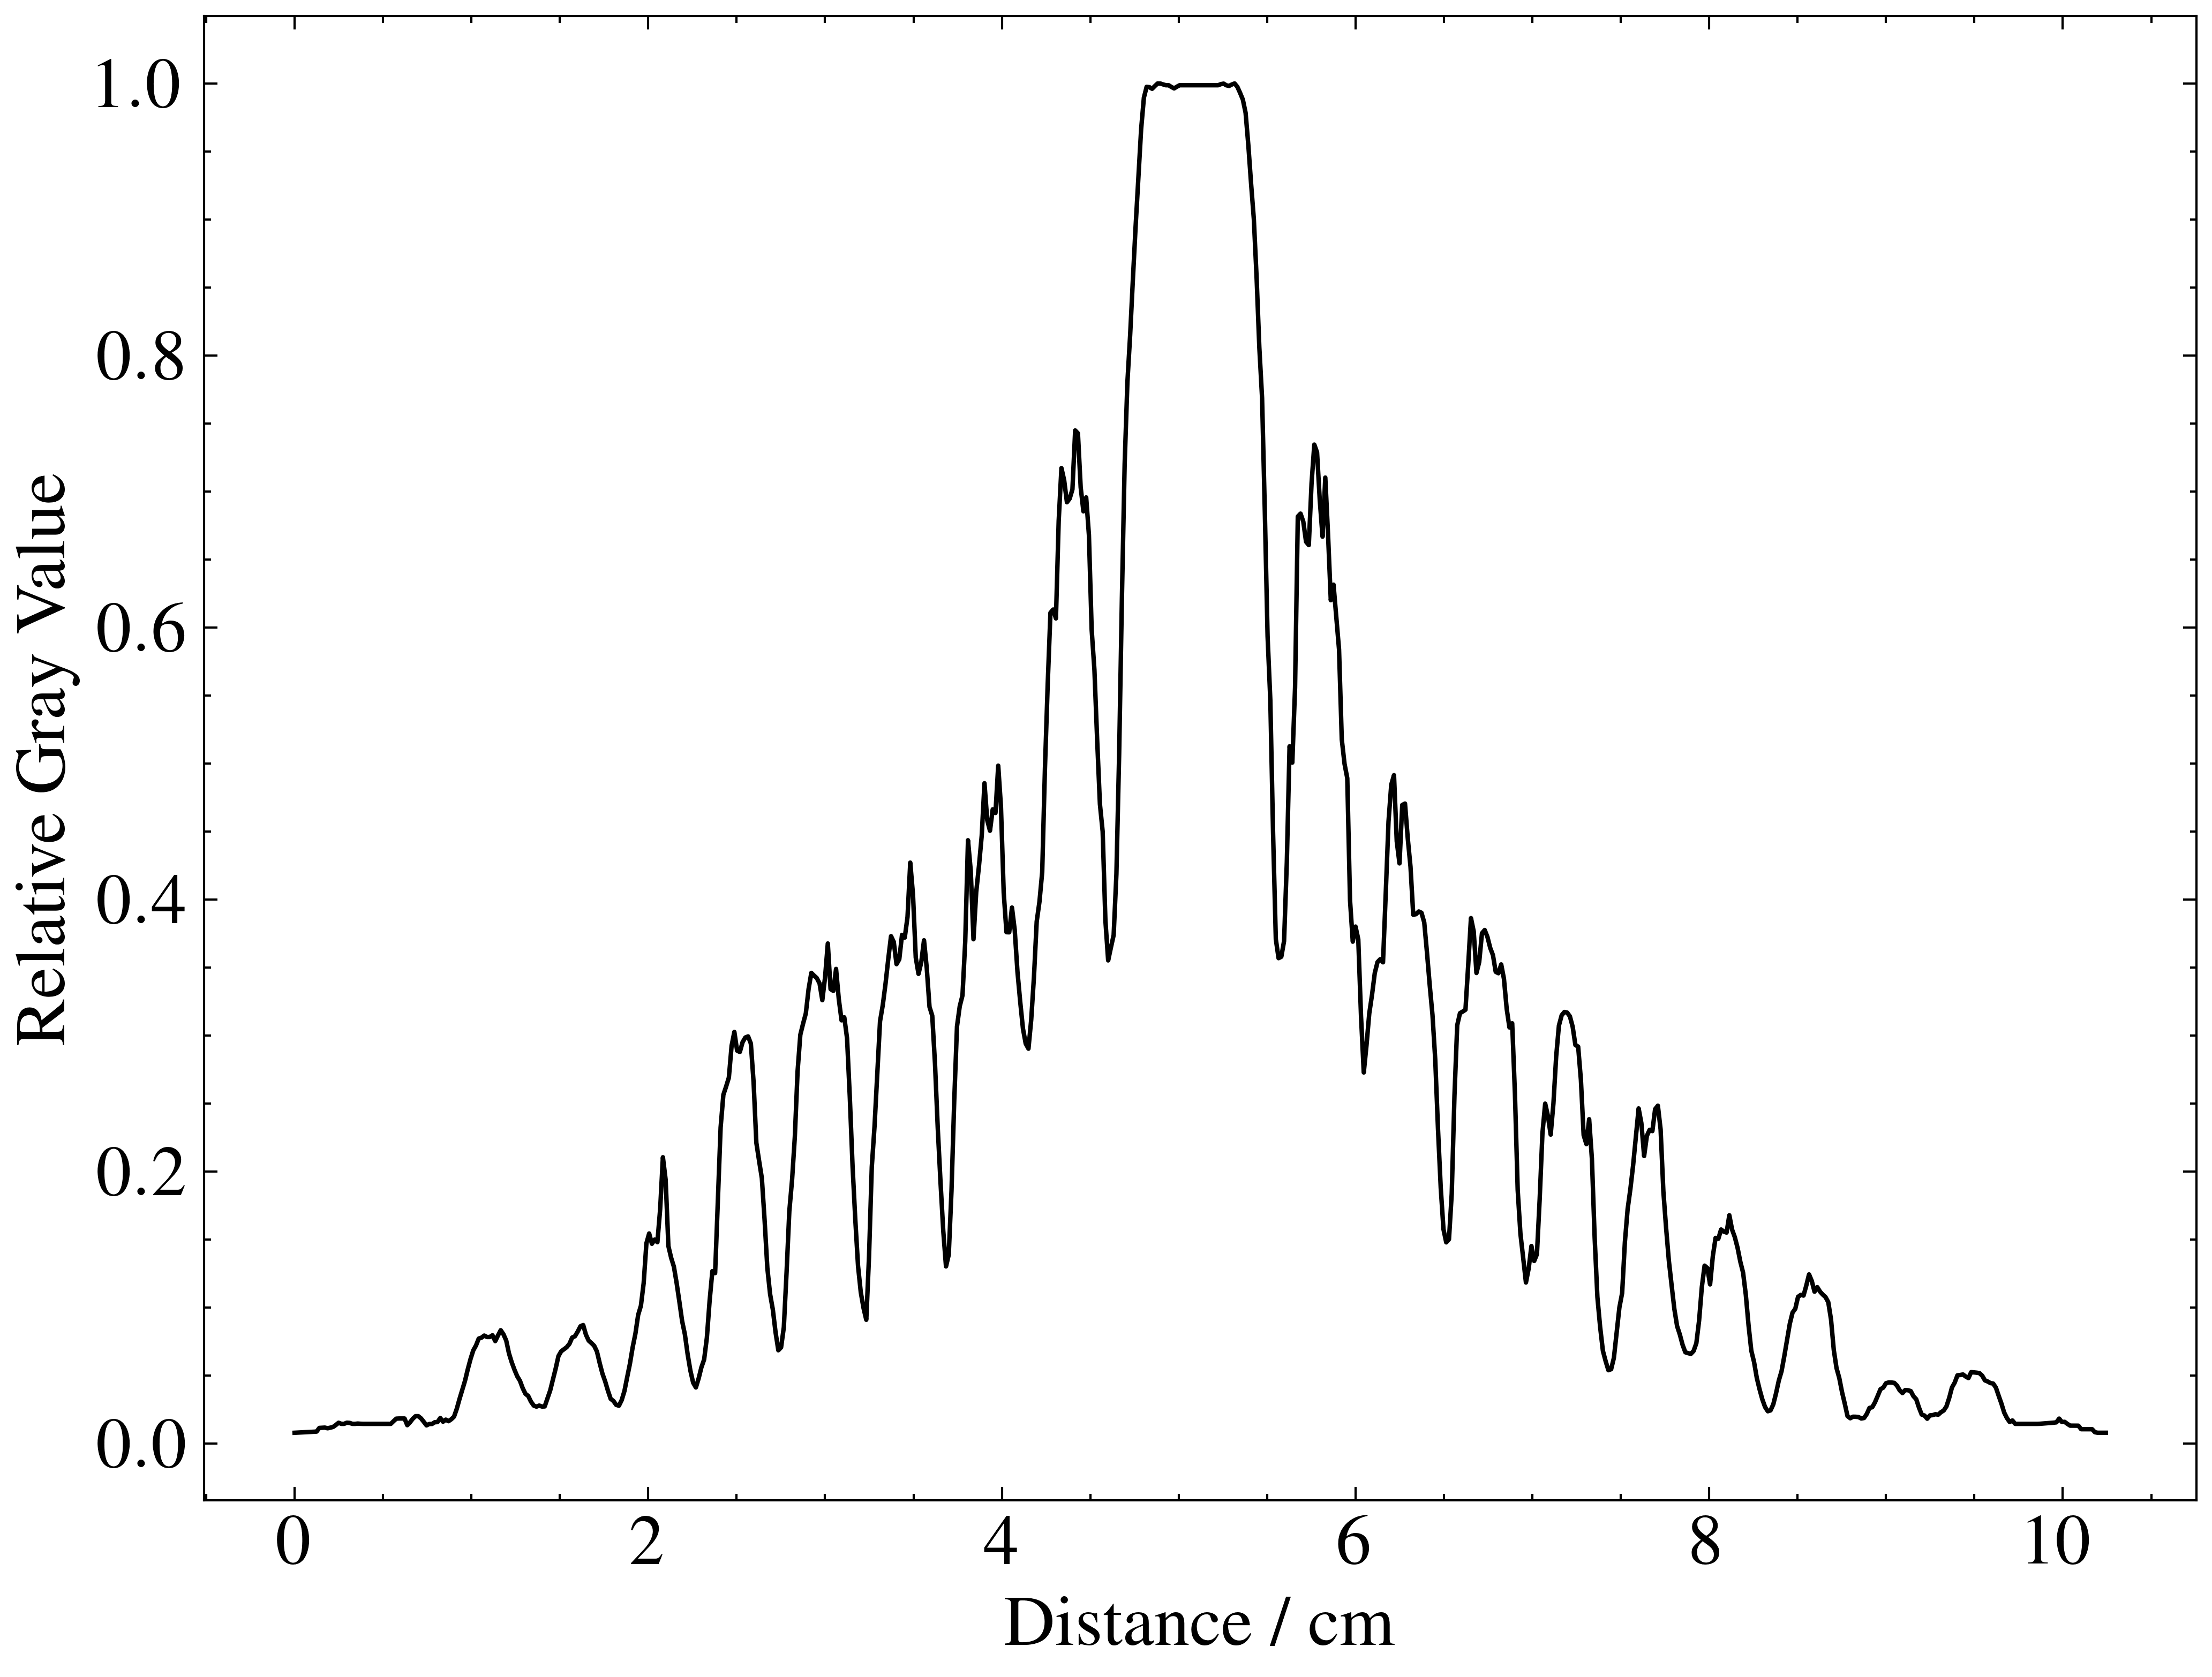
\includegraphics[width=\linewidth]{src/figures/result/ss3_data_amp.png}
		\subcaption{単スリット3}\label{subfig:ss3_amp}
	\end{minipage}
	\begin{minipage}[ht]{0.48\hsize}\centering
		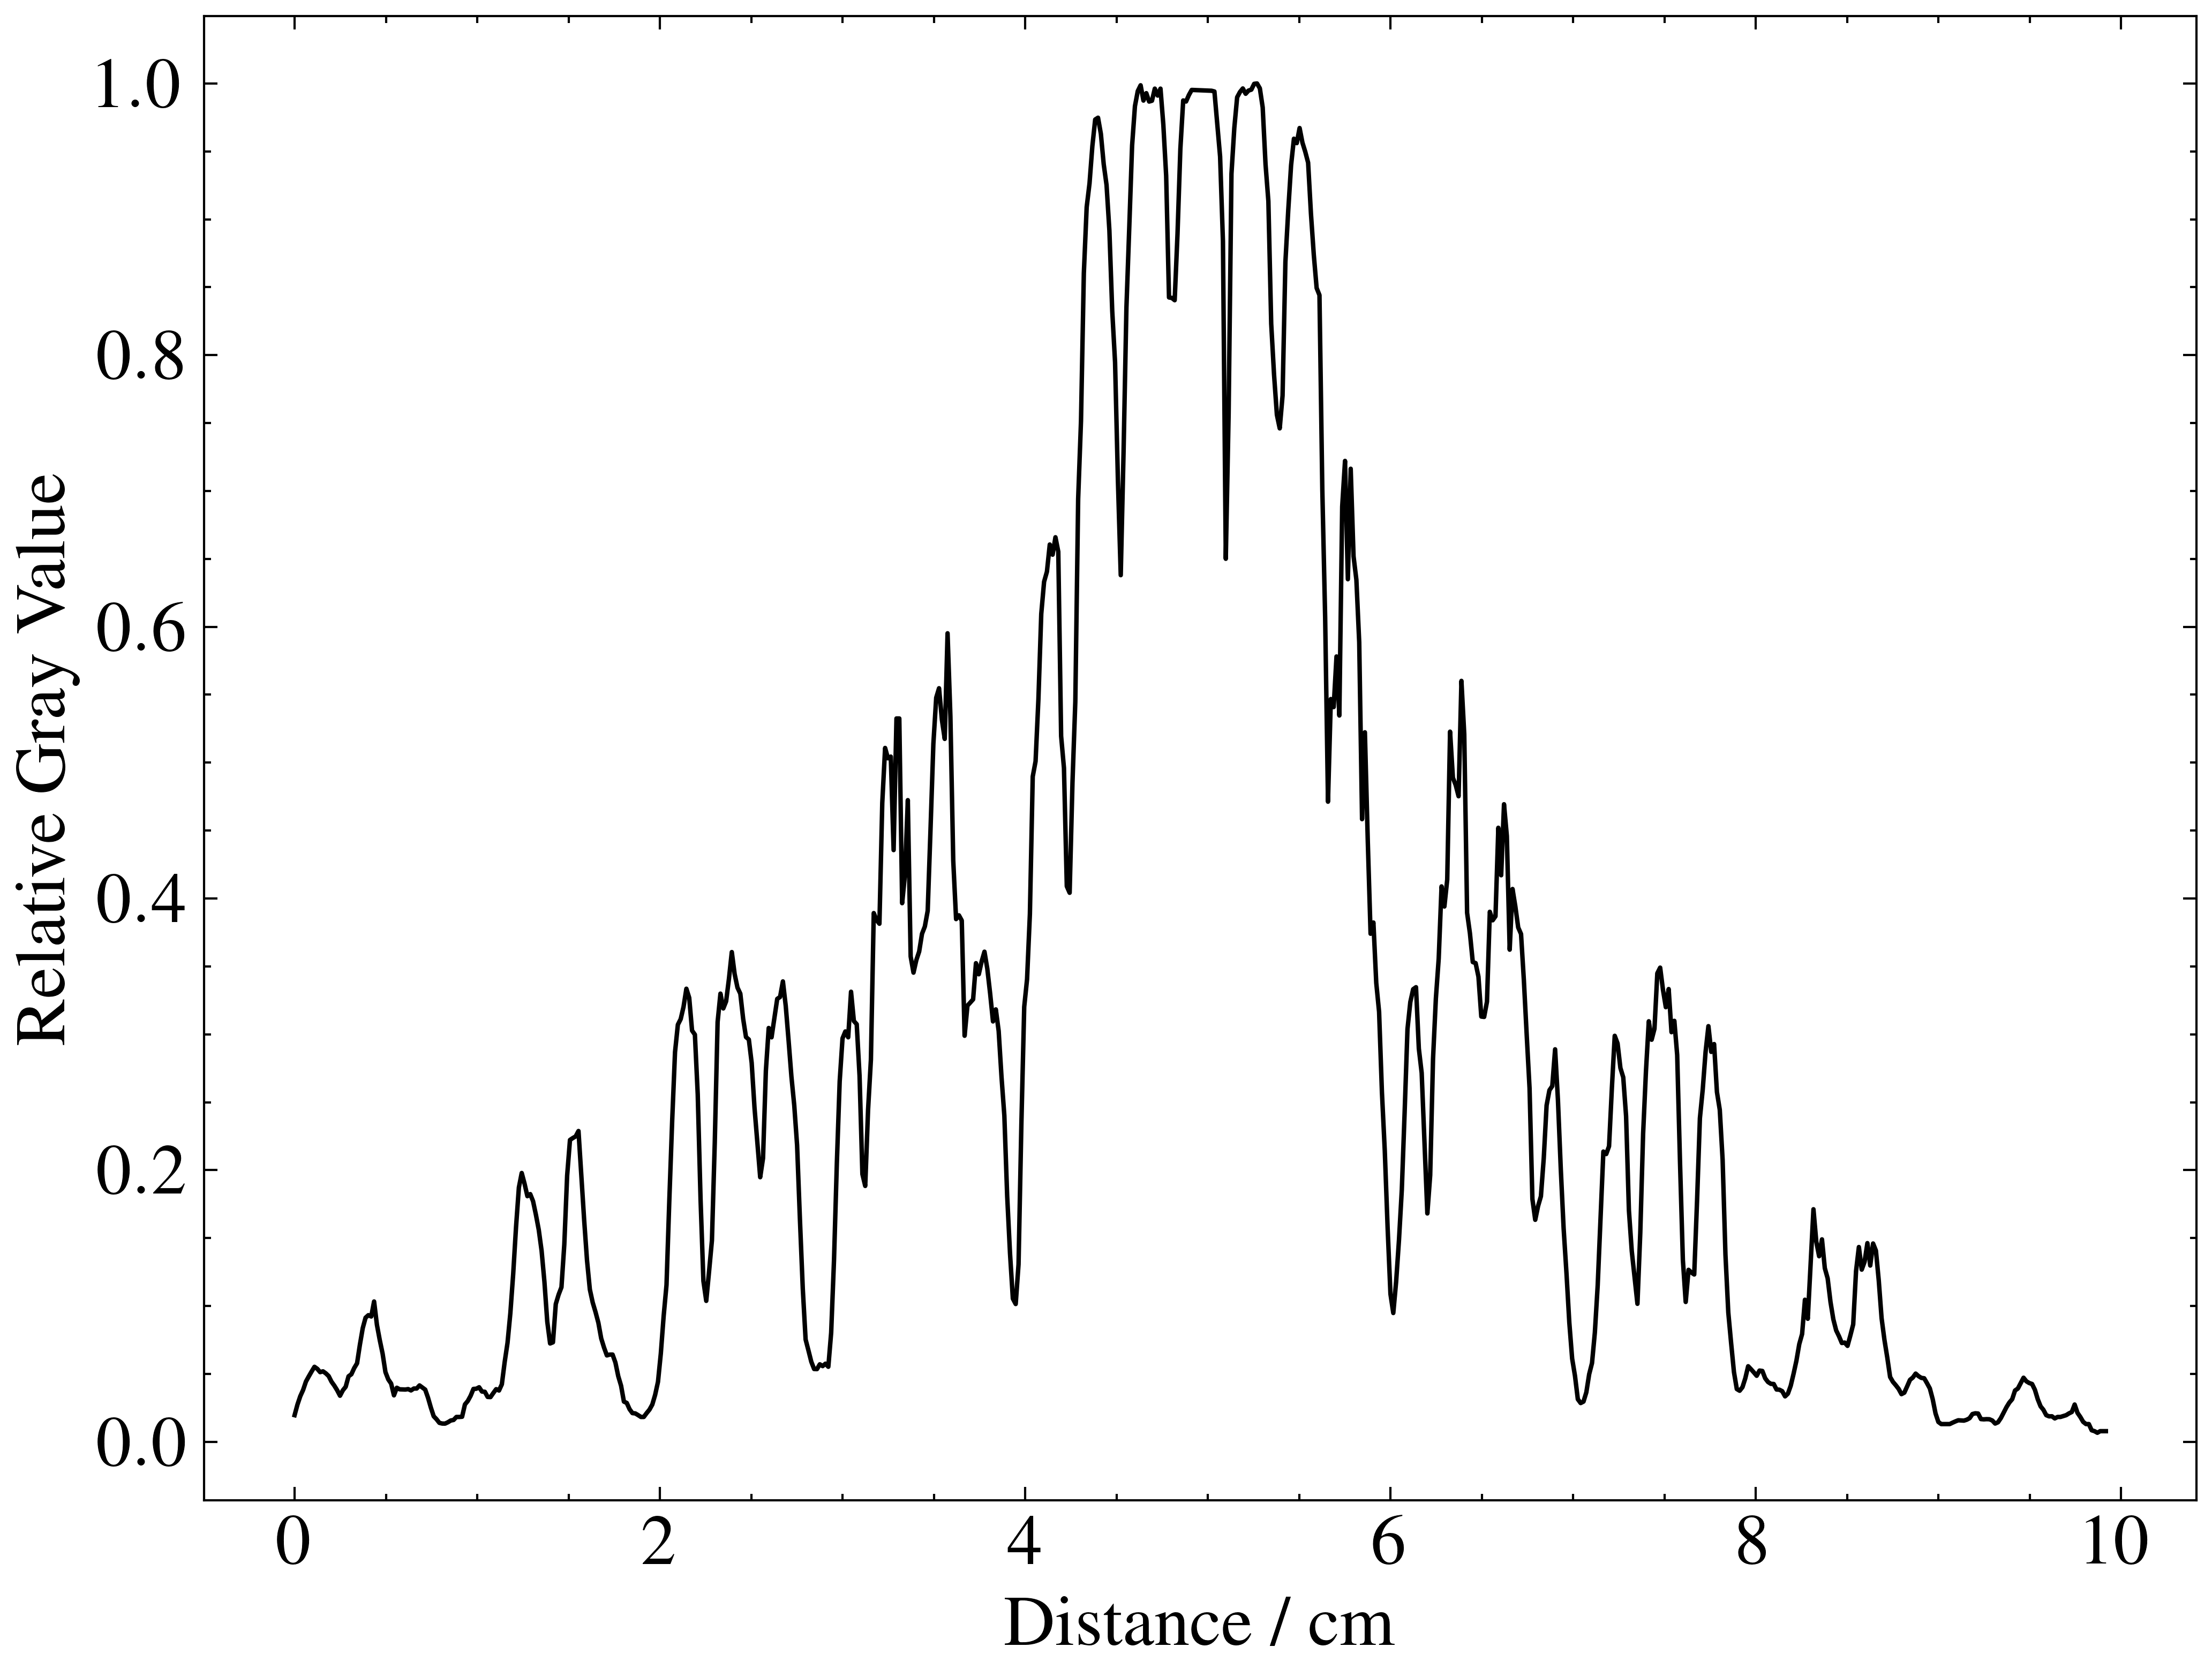
\includegraphics[width=\linewidth]{src/figures/result/ds1_data_amp.png}
		\subcaption{デュアルスリット1}\label{subfig:ds1_amp}
	\end{minipage}
	\begin{minipage}[ht]{0.48\hsize}\centering
		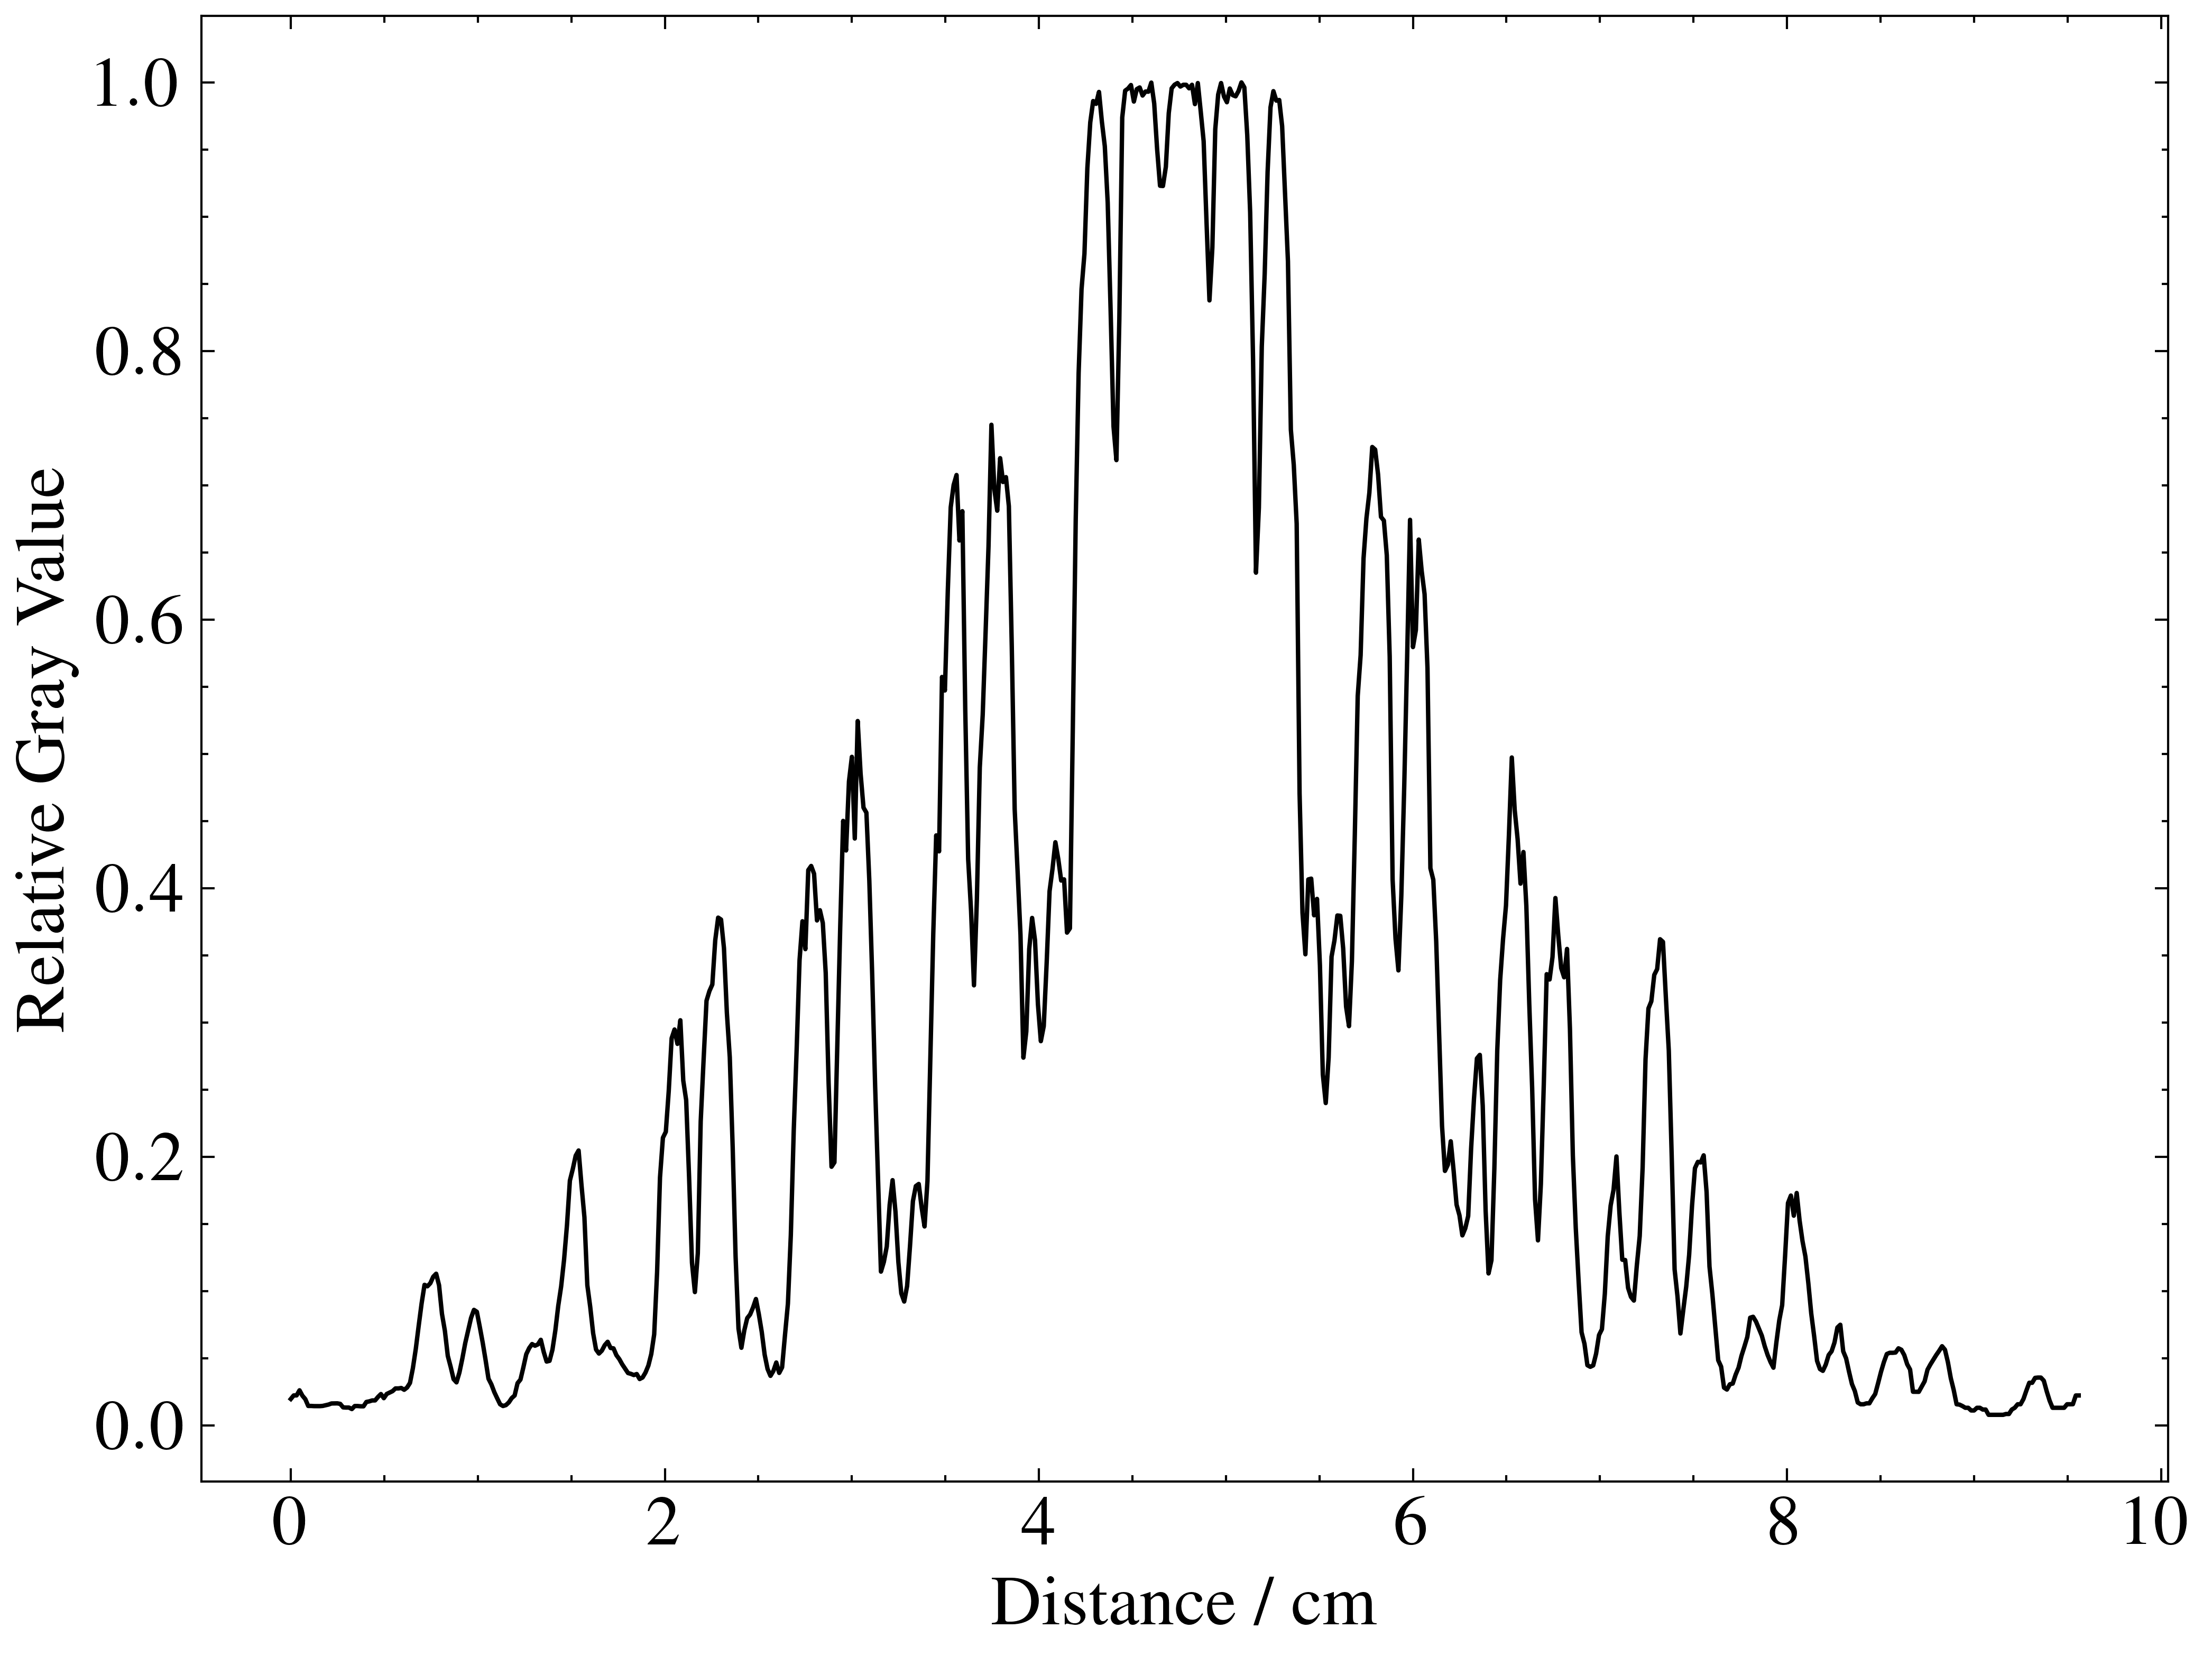
\includegraphics[width=\linewidth]{src/figures/result/ds2_data_amp.png}
		\subcaption{デュアルスリット2}\label{subfig:ds2_amp}
	\end{minipage}
\end{figure}
\begin{figure}
	\addtocounter{figure}{-1}
	\begin{subfigure}{0.48\hsize}\centering
		\addtocounter{subfigure}{6}
		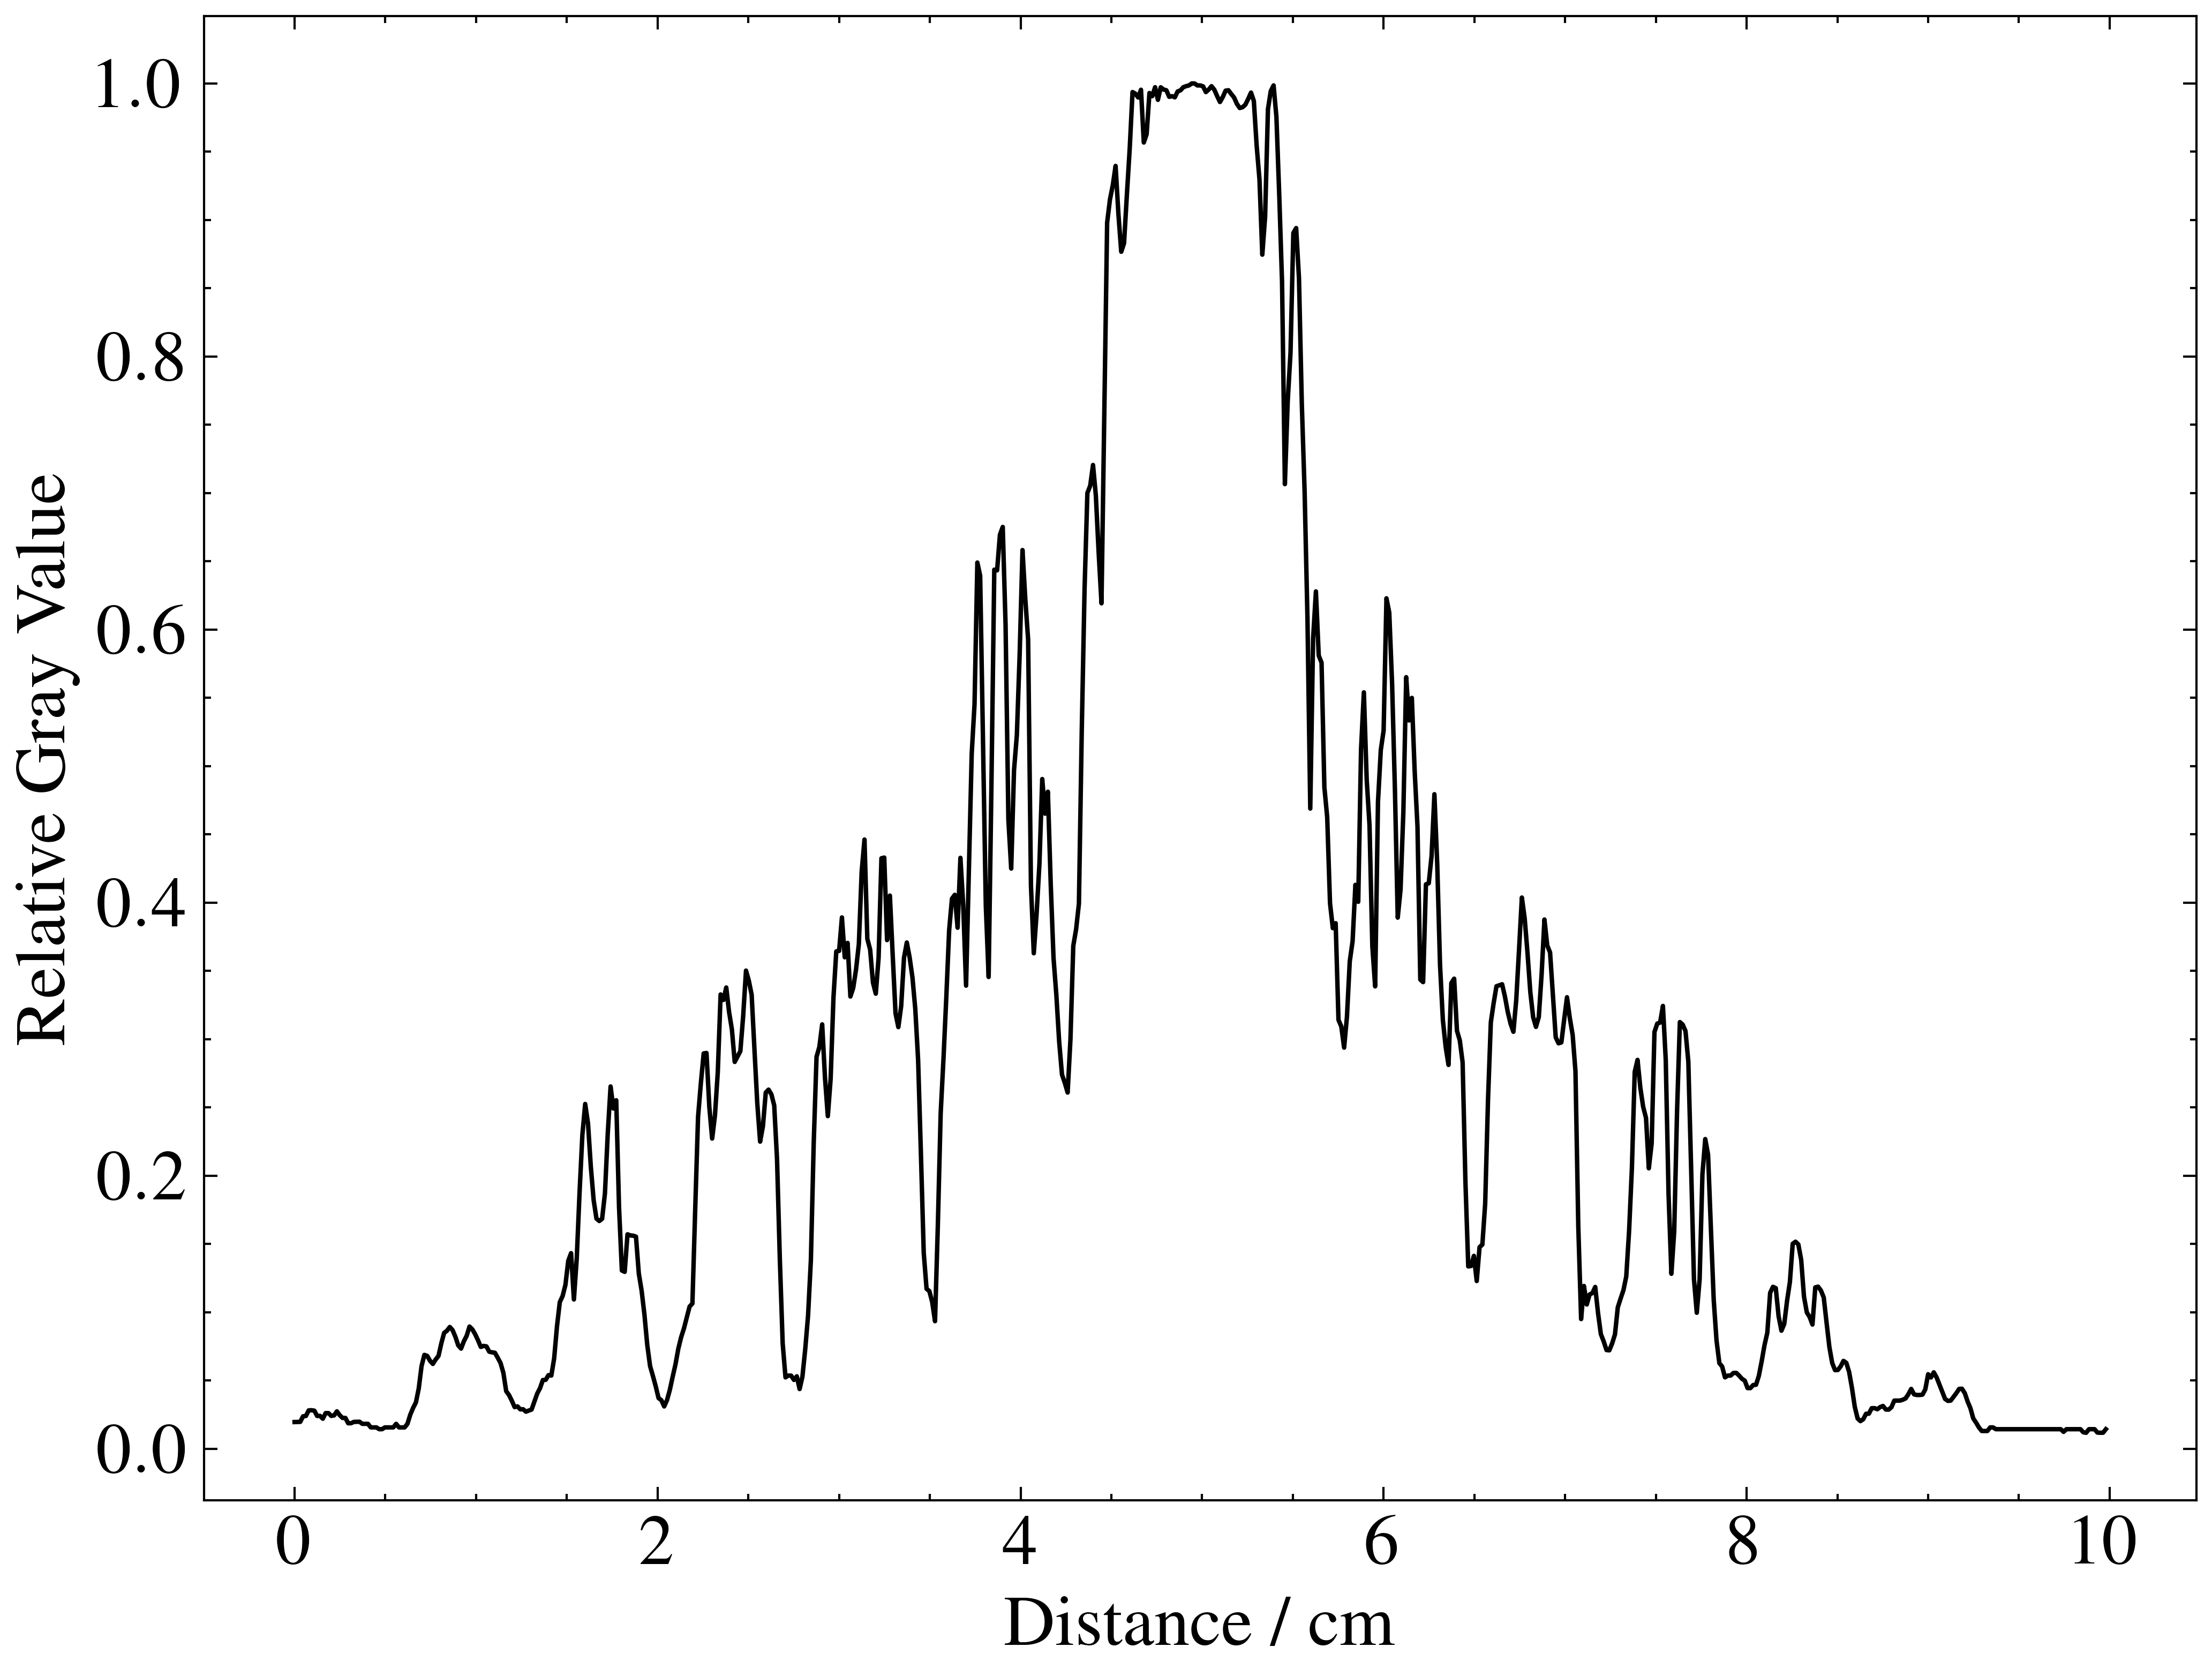
\includegraphics[width=\linewidth]{src/figures/result/ds3_data_amp.png}
		\subcaption{デュアルスリット3}\label{subfig:ds3_amp}
	\end{subfigure}
	\caption{強度分布}\label{fig:amplitude}
\end{figure}


\end{document}
